\documentclass[dvipsnames, aspectratio=169]{beamer}
\usepackage[utf8]{inputenc}
\usepackage{listings}
\usepackage{comment}
\usepackage{soul}
%\usepackage{ulem}
\usepackage{subfig}
\usepackage{pgf-pie}
\setul{}{1pt}
\usepackage[oldenum, olditem]{paralist}
%allow even smaller text
\newcommand\tinytiny{\fontsize{4pt}{3}\selectfont}

\makeatletter
\let\old@lstKV@SwitchCases\lstKV@SwitchCases
\def\lstKV@SwitchCases#1#2#3{}
\makeatother
\usepackage{lstlinebgrd}
\makeatletter
\let\lstKV@SwitchCases\old@lstKV@SwitchCases

\lst@Key{numbers}{none}{%
    \def\lst@PlaceNumber{\lst@linebgrd}%
    \lstKV@SwitchCases{#1}%
    {none:\\%
     left:\def\lst@PlaceNumber{\llap{\normalfont
                \lst@numberstyle{\thelstnumber}\kern\lst@numbersep}\lst@linebgrd}\\%
     right:\def\lst@PlaceNumber{\rlap{\normalfont
                \kern\linewidth \kern\lst@numbersep
                \lst@numberstyle{\thelstnumber}}\lst@linebgrd}%
    }{\PackageError{Listings}{Numbers #1 unknown}\@ehc}}
\makeatother


%disclaimer for Sandia. uncomment and the whole blob goes away @ b80c116300122
\def\sandid{SAND2020-7475 PE}

% \title{Performance Portability with Kokkos}
\title{The Kokkos Lectures}

%BAD misuse of author field
\author{Module 2: Views and Spaces}

%\author{
%  Jeff Miles \inst{1},
%  Christian Trott \inst{1}
%}
%\institute[shortinst]{\tiny \inst{1} Sandia National Laboratories, \inst{2} Oak Ridge National Laboratory \and \inst{3} Los Alamos National Laboratory}
%\institute[shortinst]{\tiny \inst{1} Sandia National Laboratories}

\usetheme{kokkos}

\newif\ifshort
\newif\ifmedium
\newif\iffull
\newif\ifnotoverview

\newcommand{\TutorialDirectory}{\texttt{Intro-Full}}
\newcommand{\ExerciseDirectory}[1]{\texttt{Exercises/#1/}}
\newcommand{\TutorialClone}{\texttt{Kokkos/kokkos-tutorials/\TutorialDirectory}}

\definecolor{darkgreen}{rgb}{0.0, 0.5, 0.0}
\definecolor{darkred}{rgb}{0.8, 0.0, 0.0}
\definecolor{orange}{rgb}{0.8, 0.33, 0.0}
\definecolor{purple}{rgb}{0.60, 0.20, 0.80}
\colorlet{bodyColor}{blue!20}
\colorlet{patternColor}{orange!30}
\colorlet{policyColor}{green!30}

% http://tex.stackexchange.com/questions/144448/color-a-text-line-in-a-code-lstlisting
\lstnewenvironment{code}[1][]%
{
  %with txfonts: OT1/txr/m/n/10
  %with default fonts: OT1/cmr/m/n/10
  %\fontfamily{cmr}\selectfont
  %\showthe\font
   \noindent
   \minipage{\linewidth}
   %\vspace{0.5\baselineskip}
   \lstset{mathescape, escapeinside={<@}{@>},
moredelim=**[is][{\btHL[fill=patternColor]}]{@pattern}{@pattern},
moredelim=**[is][{\btHL[fill=red!30]}]{@warning}{@warning},
moredelim=**[is][{\btHL[fill=policyColor]}]{@policy}{@policy},
moredelim=**[is][{\btHL[fill=bodyColor]}]{@body}{@body},
moredelim=**[is][{\btHL[fill=red!30]}]{@warning}{@warning},
moredelim=**[is][\color{black}]{@black}{@black},
moredelim=**[is][\color{blue}]{@blue}{@blue},
moredelim=**[is][\bf]{@bold}{@bold},
moredelim=**[is][\it]{@italic}{@italic},
moredelim=**[is][\color{boldblue}\bf]{@boldblue}{@boldblue},
moredelim=**[is][\color{red}]{@red}{@red},
moredelim=**[is][\color{green}]{@green}{@green},
moredelim=**[is][\color{gray}]{@gray}{@gray},
moredelim=**[is][\color{darkgreen}]{@darkgreen}{@darkgreen},
moredelim=**[is][\color{darkred}]{@darkred}{@darkred},
moredelim=**[is][\color{orange}]{@orange}{@orange},
moredelim=**[is][\color{purple}]{@purple}{@purple},
keywords={},
#1}
}
{
  \endminipage
  %\vspace{1.0\baselineskip}
}

\makeatletter
\newif\ifATOlinebackground
\lst@Key{linebackground}{\tiny}{\def\ATOlinebackground{#1}\global\ATOlinebackgroundtrue}
\makeatother

\lstnewenvironment{shell}[1][]{%
  \global\ATOlinebackgroundfalse
  \lstset{language=sh,%
    showstringspaces=false,
    aboveskip=0pt,
    frame=none,
    numbers=none,
    belowskip=2pt,
    breaklines=true,
    #1,
    }
  %\ifATOlinebackground
  \lstset{linebackgroundcolor={
    \ATOlinebackground
  }}
  %\fi
  }{}

\lstnewenvironment{cmake}[1][]{%
  \global\ATOlinebackgroundfalse
  \lstset{language=sh,%
    showstringspaces=false,
    aboveskip=0pt,
    frame=none,
    numbers=none,
    belowskip=2pt,
    breaklines=true,
    #1,
    }
  %\ifATOlinebackground
  \lstset{linebackgroundcolor={
    \ATOlinebackground
  }}
  %\fi
  }{}

\newcommand{\inlinecode}[1]{{\lstset{basicstyle=\ttfamily,keywordstyle={},showstringspaces=false}\lstinline$#1$}}
\newcommand{\inlineshell}[1]{{\lstset{basicstyle=\ttfamily,keywordstyle={},showstringspaces=false}\lstinline$#1$}}

\setbeamercolor{block title}{fg=white, bg=SandiaLightBlue}
\setbeamercolor{block body}{bg=lightgray}
\setbeamercolor{block title alerted}{fg=white, bg=SandiaRed}
\setbeamercolor{block body alerted}{bg=lightgray}



%\usepackage[texcoord,grid,gridunit=mm,gridcolor=red!10,subgridcolor=green!10]{eso-pic}
\usepackage[absolute,overlay]{textpos}





% http://tex.stackexchange.com/questions/8851/how-can-i-highlight-some-lines-from-source-code

\usepackage{pgf, pgffor}
\usepackage{listings}
\usepackage{lstlinebgrd} % see http://www.ctan.org/pkg/lstaddons

\makeatletter
%%%%%%%%%%%%%%%%%%%%%%%%%%%%%%%%%%%%%%%%%%%%%%%%%%%%%%%%%%%%%%%%%%%%%%%%%%%%%%
%
% \btIfInRange{number}{range list}{TRUE}{FALSE}
%
% Test in int number <number> is element of a (comma separated) list of ranges
% (such as: {1,3-5,7,10-12,14}) and processes <TRUE> or <FALSE> respectively

\newcount\bt@rangea
\newcount\bt@rangeb

\newcommand\btIfInRange[2]{%
    \global\let\bt@inrange\@secondoftwo%
    \edef\bt@rangelist{#2}%
    \foreach \range in \bt@rangelist {%
        \afterassignment\bt@getrangeb%
        \bt@rangea=0\range\relax%
        \pgfmathtruncatemacro\result{ ( #1 >= \bt@rangea) && (#1 <= \bt@rangeb) }%
        \ifnum\result=1\relax%
            \breakforeach%
            \global\let\bt@inrange\@firstoftwo%
        \fi%
    }%
    \bt@inrange%
}
\newcommand\bt@getrangeb{%
    \@ifnextchar\relax%
        {\bt@rangeb=\bt@rangea}%
        {\@getrangeb}%
}
\def\@getrangeb-#1\relax{%
    \ifx\relax#1\relax%
        \bt@rangeb=100000%   \maxdimen is too large for pgfmath
    \else%
        \bt@rangeb=#1\relax%
    \fi%
}

%%%%%%%%%%%%%%%%%%%%%%%%%%%%%%%%%%%%%%%%%%%%%%%%%%%%%%%%%%%%%%%%%%%%%%%%%%%%%%
%
% \btLstHL<overlay spec>{range list}
%
% TODO BUG: \btLstHL commands can not yet be accumulated if more than one overlay spec match.
%
\newcommand<>{\btLstHL}[2]{%
  \only#3{\btIfInRange{\value{lstnumber}}{#1}{\color{#2}\def\lst@linebgrdcmd{\color@block}}{\def\lst@linebgrdcmd####1####2####3{}}}%
}%
\makeatother






% http://tex.stackexchange.com/questions/15237/highlight-text-in-code-listing-while-also-keeping-syntax-highlighting
%\usepackage[T1]{fontenc}
%\usepackage{listings,xcolor,beramono}
\usepackage{tikz}

\makeatletter
\newenvironment{btHighlight}[1][]
{\begingroup\tikzset{bt@Highlight@par/.style={#1}}\begin{lrbox}{\@tempboxa}}
{\end{lrbox}\bt@HL@box[bt@Highlight@par]{\@tempboxa}\endgroup}

\newcommand\btHL[1][]{%
  \begin{btHighlight}[#1]\bgroup\aftergroup\bt@HL@endenv%
}
\def\bt@HL@endenv{%
  \end{btHighlight}%
  \egroup
}
\newcommand{\bt@HL@box}[2][]{%
  \tikz[#1]{%
    \pgfpathrectangle{\pgfpoint{1pt}{0pt}}{\pgfpoint{\wd #2}{\ht #2}}%
    \pgfusepath{use as bounding box}%
    \node[anchor=base west, fill=orange!30,outer sep=0pt,inner xsep=1pt, inner ysep=0pt, rounded corners=3pt, minimum height=\ht\strutbox+1pt,#1]{\raisebox{1pt}{\strut}\strut\usebox{#2}};
  }%
}
\makeatother



\usetikzlibrary{calc}
\usepackage{xparse}%  For \NewDocumentCommand

% tikzmark command, for shading over items
\newcommand{\tikzmark}[1]{\tikz[overlay,remember picture] \node (#1) {};}

\makeatletter
\NewDocumentCommand{\DrawBox}{s O{}}{%
    \tikz[overlay,remember picture]{
    \IfBooleanTF{#1}{%
        \coordinate (RightPoint) at ($(left |- right)+(\linewidth-\labelsep-\labelwidth,0.0)$);
    }{%
        \coordinate (RightPoint) at (right.east);
    }%
    \draw[red,#2]
      ($(left)+(-0.2em,0.9em)$) rectangle
      ($(RightPoint)+(0.2em,-0.3em)$);}
}

\NewDocumentCommand{\DrawBoxWide}{s O{}}{%
    \tikz[overlay,remember picture]{
    \IfBooleanTF{#1}{%
        \coordinate (RightPoint) at ($(left |- right)+(\linewidth-\labelsep-\labelwidth,0.0)$);
    }{%
        \coordinate (RightPoint) at (right.east);
    }%
    \draw[red,#2]
      ($(left)+(-\labelwidth,0.9em)$) rectangle
      ($(RightPoint)+(0.2em,-0.3em)$);}
}

\NewDocumentCommand{\DrawBoxWideBlack}{s O{}}{%
    \tikz[overlay,remember picture]{
    \IfBooleanTF{#1}{%
        \coordinate (RightPoint) at ($(left |- right)+(\linewidth-\labelsep-\labelwidth,0.0)$);
    }{%
        \coordinate (RightPoint) at (right.east);
    }%
    \draw[black,#2]
      ($(left)+(-\labelwidth,0.9em)$) rectangle
      ($(RightPoint)+(0.2em,-0.3em)$);}
}
\makeatother

\usetikzlibrary{positioning}

\usetikzlibrary{shapes}

\hypersetup{
    colorlinks=true,
    linkcolor=blue,
    filecolor=magenta,
    urlcolor=cyan,
}



\shortfalse
\mediumtrue
\fulltrue
\notoverviewtrue

\begin{document}

% \begin{frame}
%   \titlepage
% \end{frame}
% 
%==============================================================================

\begin{frame}{NVIDIA's NVLABS LOGISTICS (1)}

\textbf{\large SOFTWARE FOR LAB}

\vspace{10pt}

\textbf{Remote Desktop Software:} \\
\begin{itemize}
\item {Download NoMachine now for best performance from \\
 \textbf{\ul{www.nomachine.com/download}}}
\item {Alternatively you may use a VNC client or the provided browser-based VNC option}
\end{itemize}

\vspace{10pt}

\textbf{SSH Access Software (optional):}
\begin{itemize}
\item PuTTy for Windows can be downloaded from \textbf{\ul{www.putty.org}}
\item{Alternatively you may use a provided browser-based SSH option}
\end{itemize}

\end{frame}

%==============================================================================

\begin{frame}{NVIDIA's NVLABS LOGISTICS (2)}

\textbf{\Large CONNECTION INSTRUCTIONS}
\begin{itemize}
\item {Navigate to \textbf{\ul{nvlabs.qwiklab.com}}}
\item {Login or create a new account}
\item {Select the \textbf{Instructor-Led Hands-on Labs} Class}
\item {Find the lab called \textbf{Kokkos, ...}, select it, click Select, and finally click Start}
\item {After a short wait, lab instance Connection information will be shown}
\item {Please ask Lab Assistants for help!}
\end{itemize}

\end{frame}

%==============================================================================



\begin{frame}
	\titlepage
\end{frame}

\begin{frame}{Welcome to Kokkos}

\textbf{Online Resources}:

\begin{itemize}
        \item \url{https://github.com/kokkos}:
                \begin{itemize}
                        \item Primary Kokkos GitHub Organization
                \end{itemize}
        \item \url{https://kokkos.org/kokkos-core-wiki/videolectures.html}
                \begin{itemize}
			\item{Slides, recording and Q\&A for the lectures}
                \end{itemize}
        \item \url{https://kokkos.org/kokkos-core-wiki}:
                \begin{itemize}
                        \item Programming guide and API reference documentation
                \end{itemize}
        \item \url{https://kokkosteam.slack.com}:
                \begin{itemize}
                        \item Slack channel for Kokkos.
                        \item Please join: fastest way to get your questions answered.
                        \item Can whitelist domains, or invite individual people.
                \end{itemize}
\end{itemize}

\end{frame}


\begin{frame}{Lecture Series Outline}

\begin{itemize}
        \item Module 1: Introduction, Building and Parallel Dispatch
        \item \textbf{Module 2: Views and Spaces}
        \item Module 3: Data Structures + MultiDimensional Loops
        \item Module 4: Hierarchical Parallelism
        \item Module 5: Tasking, Streams and SIMD
        \item Module 6: Internode: MPI and PGAS
        \item Module 7: Tools: Profiling, Tuning and Debugging
        \item Module 8: Kernels: Sparse and Dense Linear Algebra
        \item Module 9: Fortran inter-op
\end{itemize}
\end{frame}

\begin{frame}{Module 1: Summary}
	\textbf{Kokkos Ecosystem:}
	\begin{itemize}
		\item C++ Performance Portability Programming Model.
		\item The Kokkos Ecosystem provides capabilities needed for serious code development.
		\item Kokkos is supported by multiple National Laboratories with a sizeable dedicated team.
	\end{itemize}

	\textbf{Building Kokkos}
	\begin{itemize}
    \item{Kokkos's primary build system is CMAKE.}
    \item{Kokkos options are transitively passed on, including many necessary compiler options.}
    \item{The Spack package manager does support Kokkos.}
    \item{For applications with few if any dependencies, building Kokkos as part of your code is an option with CMake and GNU Makefiles.}
	\end{itemize}
\end{frame}

\begin{frame}[fragile]{Module 1: Summary}
	\textbf{Data Parallelism:}
	\begin{itemize}
		\item Simple things stay simple!
		\item You use \textbf{parallel patterns} and \textbf{execution policies} to execute \textbf{computational bodies}
		\item Simple parallel loops use the \texttt{parallel\_for} pattern:
\begin{code}[linebackgroundcolor={\btLstHL<1->{3}{bodyColor}},frame=single]
  @patternparallel_for@pattern("Label",@policyN@policy, [=] (int64_t i) {
   /* loop body */
  });
\end{code}
\item Reductions combine contributions from loop iterations
\begin{code}[linebackgroundcolor={\btLstHL<1->{3}{bodyColor}},frame=single]
int result;
@patternparallel_reduce@pattern("Label",@policyN@policy, [=] (int64_t i, int& lres) {
   /* loop body */
    lres += /* something */
  },result);
\end{code}

\end{itemize}

	\textbf{Recording:} \url{https://bit.ly/kokkos-lecture-series-1}

\end{frame}

\begin{frame}{Module 2}
  \begin{block}{Kokkos View}
    What are Views? How to create them? Why should you use it?
  \end{block}


  \begin{block}{Memory and Execution Spaces}
    How to control where data lives and code executes.
  \end{block}

  \begin{block}{Memory Access Patterns}
    The importance of access patterns for performance portability and how to control it.
  \end{block}

  \begin{block}{Advanced Reductions}
    Going beyond just basic summation.
  \end{block}
\end{frame}  

%==========================================================================

\begin{frame}[fragile]

  {\Huge Views}

  \vspace{20pt}

  \textbf{Learning objectives:}
  \begin{itemize}
    \item{Motivation behind the \texttt{View} abstraction.}
    \item{Key \texttt{View} concepts and template parameters.}
    \item{The \texttt{View} life cycle.}
  \end{itemize}

  \vspace{-20pt}

\end{frame}

%==========================================================================

\begin{frame}[fragile]{View motivation}

  \textbf{\ul{Example: running \texttt{daxpy} on the GPU:}}

  \vspace{5pt}

  \begin{code}[linebackgroundcolor={
        \btLstHL<2->{3}{red!30}
      },
      frame=single
    ]
double * x = new double[N]; // also y
parallel_for("DAXPY",N, [=] (const int64_t i) {
    y[i] = a * x[i] + y[i];
  });
  \end{code}

  \begin{code}[linebackgroundcolor={
        \btLstHL<2->{2,4}{red!30}
      },
      frame=single
    ]
struct Functor {
  double *_x, *_y, a;
  void operator()(const int64_t i) const {
    _y[i] = _a * _x[i] + _y[i];
  }
};
  \end{code}

  \begin{textblock*}{0.5\textwidth}(0.05\textwidth,0.225\textheight)
    \rotatebox{90}{\textbf{Lambda}}
  \end{textblock*}

  \begin{textblock*}{0.5\textwidth}(0.05\textwidth,0.470\textheight)
    \rotatebox{90}{\textbf{Functor}}
  \end{textblock*}

  \vspace{5pt}
  \pause

  \textbf{{\color{red}Problem}}: \texttt{x} and \texttt{y} reside in CPU memory.

  \vspace{5pt}
  \pause

  \textbf{Solution:} We need a way of storing data (multidimensional arrays) which can be communicated to an accelerator (GPU).

  \vspace{5pt}

  \hspace{20pt}{\Large $\Rightarrow$ \textbf{Views}}

  \vspace{-5pt}

\end{frame}

%==========================================================================

\begin{frame}[fragile]{Views (0)}

  \ul{\textbf{View} abstraction}
  \begin{itemize}
  \item {A \textit{lightweight} C++ class with a pointer to array data and a little meta-data,}
  \item {that is \textit{templated} on the data type (and other things).}
  \end{itemize}

  \vspace{5pt}

  \ul{\textbf{High-level example} of Views for \texttt{daxpy} using lambda}:

  \begin{code}[frame=single, keywords={}]
@blueView<double*, ...>@blue x(...), y(...);
@gray...populate x, y... @gray

parallel_for("DAXPY",N, [=] (const int64_t i) {
    // Views x and y are captured by value (shallow copy)
    y(i) = a * x(i) + y(i);
  });
  \end{code}

  \pause
  \vspace{0pt}

  \begin{block}{Important point}
    Views are \textbf{like pointers}, so copy them in your functors.
  \end{block}

  \vspace{5pt}

\end{frame}

%==========================================================================

\begin{frame}[fragile]{Views (1)}

  \ul{\textbf{View} overview:}

  \begin{itemize}
    \item{\textbf{Multi-dimensional array} of 0 or more dimensions \\
          \hspace{20pt}scalar (0), vector (1), matrix (2), etc.}
    \item{\textbf{Number of dimensions (rank)} is fixed at compile-time.}
    \item{Arrays are \textbf{rectangular}, not ragged.}
    \item{\textbf{Sizes of dimensions} set at compile-time or runtime. \\
          \hspace{20pt}e.g., 2x20, 50x50, etc.}
    \item{Access elements via "(...)" operator.}
  \end{itemize}

  \pause
  \vspace{-3pt}

  \textbf{Example}:
  \vspace{-3pt}
  \begin{code}[keywords={double,View}]
View<double***> data("label", N0, N1, N2); //<@3 run, 0 compile@>
View<double**[N2]> data("label", N0, N1);  //<@2 run, 1 compile@>
View<double*[N1][N2]> data("label", N0);   //<@1 run, 2 compile@>
View<double[N0][N1][N2]> data("label");    //<@0 run, 3 compile@>
//Access
data(i,j,k) = 5.3;
  \end{code}

  \vspace{-1pt}
  Note: runtime-sized dimensions must come first.

\end{frame}

%==========================================================================

\begin{frame}[fragile]{Views (2)}

  \ul{\textbf{View} life cycle:}

  \begin{itemize}
    \item{Allocations only happen when \emph{explicitly} specified. \\
          \hspace{20pt}i.e., there are \textbf{no hidden allocations}.}
    \item{Copy construction and assignment are \textbf{shallow} (like pointers).\\
          \hspace{20pt}so, you pass \texttt{Views} by value, \emph{not} by reference}
    \item{Reference counting is used for \textbf{automatic deallocation.}}
    \item{They behave like \texttt{std::shared\_ptr}}
  \end{itemize}

  \pause
  \textbf{Example}:

  \vspace{-3pt}

  \begin{code}[keywords={}]
View<double*[5]> @bluea@blue("a", N), @darkgreenb@darkgreen("b", K);
@bluea@blue = @darkgreenb@darkgreen;
View<double**> @darkredc@darkred(@darkgreenb@darkgreen);
@bluea@blue(0,2) = 1;
@darkgreenb@darkgreen(0,2) = 2;
@darkredc@darkred(0,2) = 3;
print_value( @bluea@blue(0,2) );
  \end{code}

  \begin{textblock*}{0.5\textwidth}(0.6\textwidth,0.78\textheight)
    \onslide<2->{What gets printed?}
  \end{textblock*}

  \begin{textblock*}{0.5\textwidth}(0.65\textwidth,0.83\textheight)
    \onslide<3->{\texttt{3.0}}
  \end{textblock*}

\end{frame}

%==========================================================================

\begin{frame}[fragile]{Views (3)}

  \ul{\textbf{View} Properties:}

  \begin{itemize}
    \item Accessing a \texttt{View}'s sizes is done via its \texttt{extent(dim)} function.
         \begin{itemize}
		 \item Static extents can \emph{additionally} be accessed via \texttt{static\_extent(dim)}.
	 \end{itemize}
    \item You can retrieve a raw pointer via its \texttt{data()} function.
    \item The label can be accessed via \texttt{label()}.
  \end{itemize}

  \textbf{Example}:

  \begin{code}[keywords={View,extent,static_extent,data,label}]
	  View<double*[5]> a("A",N0);
	  assert(a.extent(0) == N0);
	  assert(a.extent(1) == 5);
	  static_assert(a.static_extent(1) == 5);
	  assert(a.data() != nullptr);
	  assert(a.label() == "A");
  \end{code}

\end{frame}
%==========================================================================

\begin{frame}[fragile]{Exercise \#2: Inner Product, Flat Parallelism on the CPU, with Views}

  \begin{small}
  \begin{itemize}
  \item Location: \ExerciseDirectory{02/Begin}
  \item Assignment: Change data storage from arrays to Views.
  \item Compile and run on CPU, and then on GPU with UVM
  \end{itemize}
  \end{small}

\begin{code}
# CPU-only using OpenMP
cmake -B build_openmp -DKokkos_ENABLE_OPENMP=ON
cmake --build build_openmp
# Run exercise
./build_openmp/02_Exercise -S 26
# Note the warnings, set appropriate environment variables
\end{code}

  \begin{scriptsize}
  \begin{itemize}
  \item Vary problem size: \textbf{-S \#}
  \item Vary number of rows: \textbf{-N \#}
  \item Vary repeats: \textbf{-nrepeat \#}
  \item Compare performance of CPU vs GPU
  \end{itemize}
  \end{scriptsize}

\end{frame}

%==========================================================================

\iffull
\begin{frame}[fragile]{Advanced features we haven't covered}

  \begin{itemize}

  \item {\textbf{Memory space} in which view's data resides;
         \textit{covered next}.}

  \item {\textbf{deep\_copy} view's data; \textit{covered later}. \\
        Note: Kokkos \textit{never} hides a deep\_copy of data.}

  \item {\textbf{Layout} of multidimensional array; \textit{covered later}.}

  \item {\textbf{Memory traits}; \textit{covered later}.}

  \item {\textbf{Subview}: Generating a view that is a ``slice'' of other multidimensional array view; \textit{covered later}.}

  \end{itemize}

\end{frame}
\fi



\ifmedium
\begin{frame}[fragile]{Execution and Memory spaces}

  {\Huge Execution and Memory Spaces}

  \vspace{20pt}

  \textbf{Learning objectives:}
  \begin{itemize}
    \item{Heterogeneous nodes and the \textbf{space} abstractions.}
    \item{How to control where parallel bodies are run, \textbf{execution space}.}
    \item{How to control where view data resides, \textbf{memory space}.}
    \item{How to avoid illegal memory accesses and manage data movement.}
    \item{The need for \texttt{Kokkos::initialize} and \texttt{finalize}.}
    \item{Where to use Kokkos annotation macros for portability.}
  \end{itemize}

  \vspace{-20pt}

\end{frame}
\fi

%==========================================================================

%\begin{frame}[fragile]{Execution spaces (0)}
%
%  \textbf{Thought experiment}: Consider this code:
%
%  \vspace{5pt}
%
%  \lstset{mathescape, escapeinside={<@}{@>},
%          language=C,
%          keywords={}}
%
%  \begin{lstlisting}[linebackgroundcolor={
%        \btLstHL{1-3}{darkred!20}
%      }
%    ]
%  MPI_Reduce(...);
%  FILE * file = fopen(...);
%  runANormalFunction(...data...);
%  \end{lstlisting}
%
%  \vspace{-11pt}
%
%  \begin{lstlisting}[linebackgroundcolor={
%        \btLstHL{3-4}{bodyColor}
%      }
%    ]
%  Kokkos::parallel_for(numberOfSomethings,
%                       [=] (const int64_t somethingIndex) {
%                         const double y = ...;
%                         // do something interesting
%                       }
%                       );
%  \end{lstlisting}
%
%  \begin{textblock*}{0.5\textwidth}(0.08\textwidth,0.235\textheight)
%    \rotatebox{90}{{\footnotesize {\color{darkred!80} section 1}}}
%  \end{textblock*}
%
%  \begin{textblock*}{0.5\textwidth}(0.08\textwidth,0.40\textheight)
%    \rotatebox{90}{{\footnotesize {\color{blue!80} section 2}}}
%  \end{textblock*}
%
%  \pause
%
%  \begin{itemize}
%    \item{Where will {\color{darkred!80}section 1} be run?  CPU?  GPU?}
%    \item{Where will {\color{blue!80}section 2} be run?  CPU?  GPU?}
%    \item{How do I \textbf{control} where code is executed?}
%  \end{itemize}
%
%  \pause
%  \vspace{5pt}
%
%  \hspace{20pt}{\Large $\Rightarrow$ \textbf{Execution spaces}}
%
%\end{frame}

%==========================================================================

\begin{frame}{Execution spaces (1)}

  \vspace{-15pt}

  \begin{center}
  \textbf{Execution Space} \\
  a homogeneous set of cores and an execution mechanism \\
  (i.e., ``place to run code'')
  \end{center}

  \vspace{-15pt}

  \begin{center}
    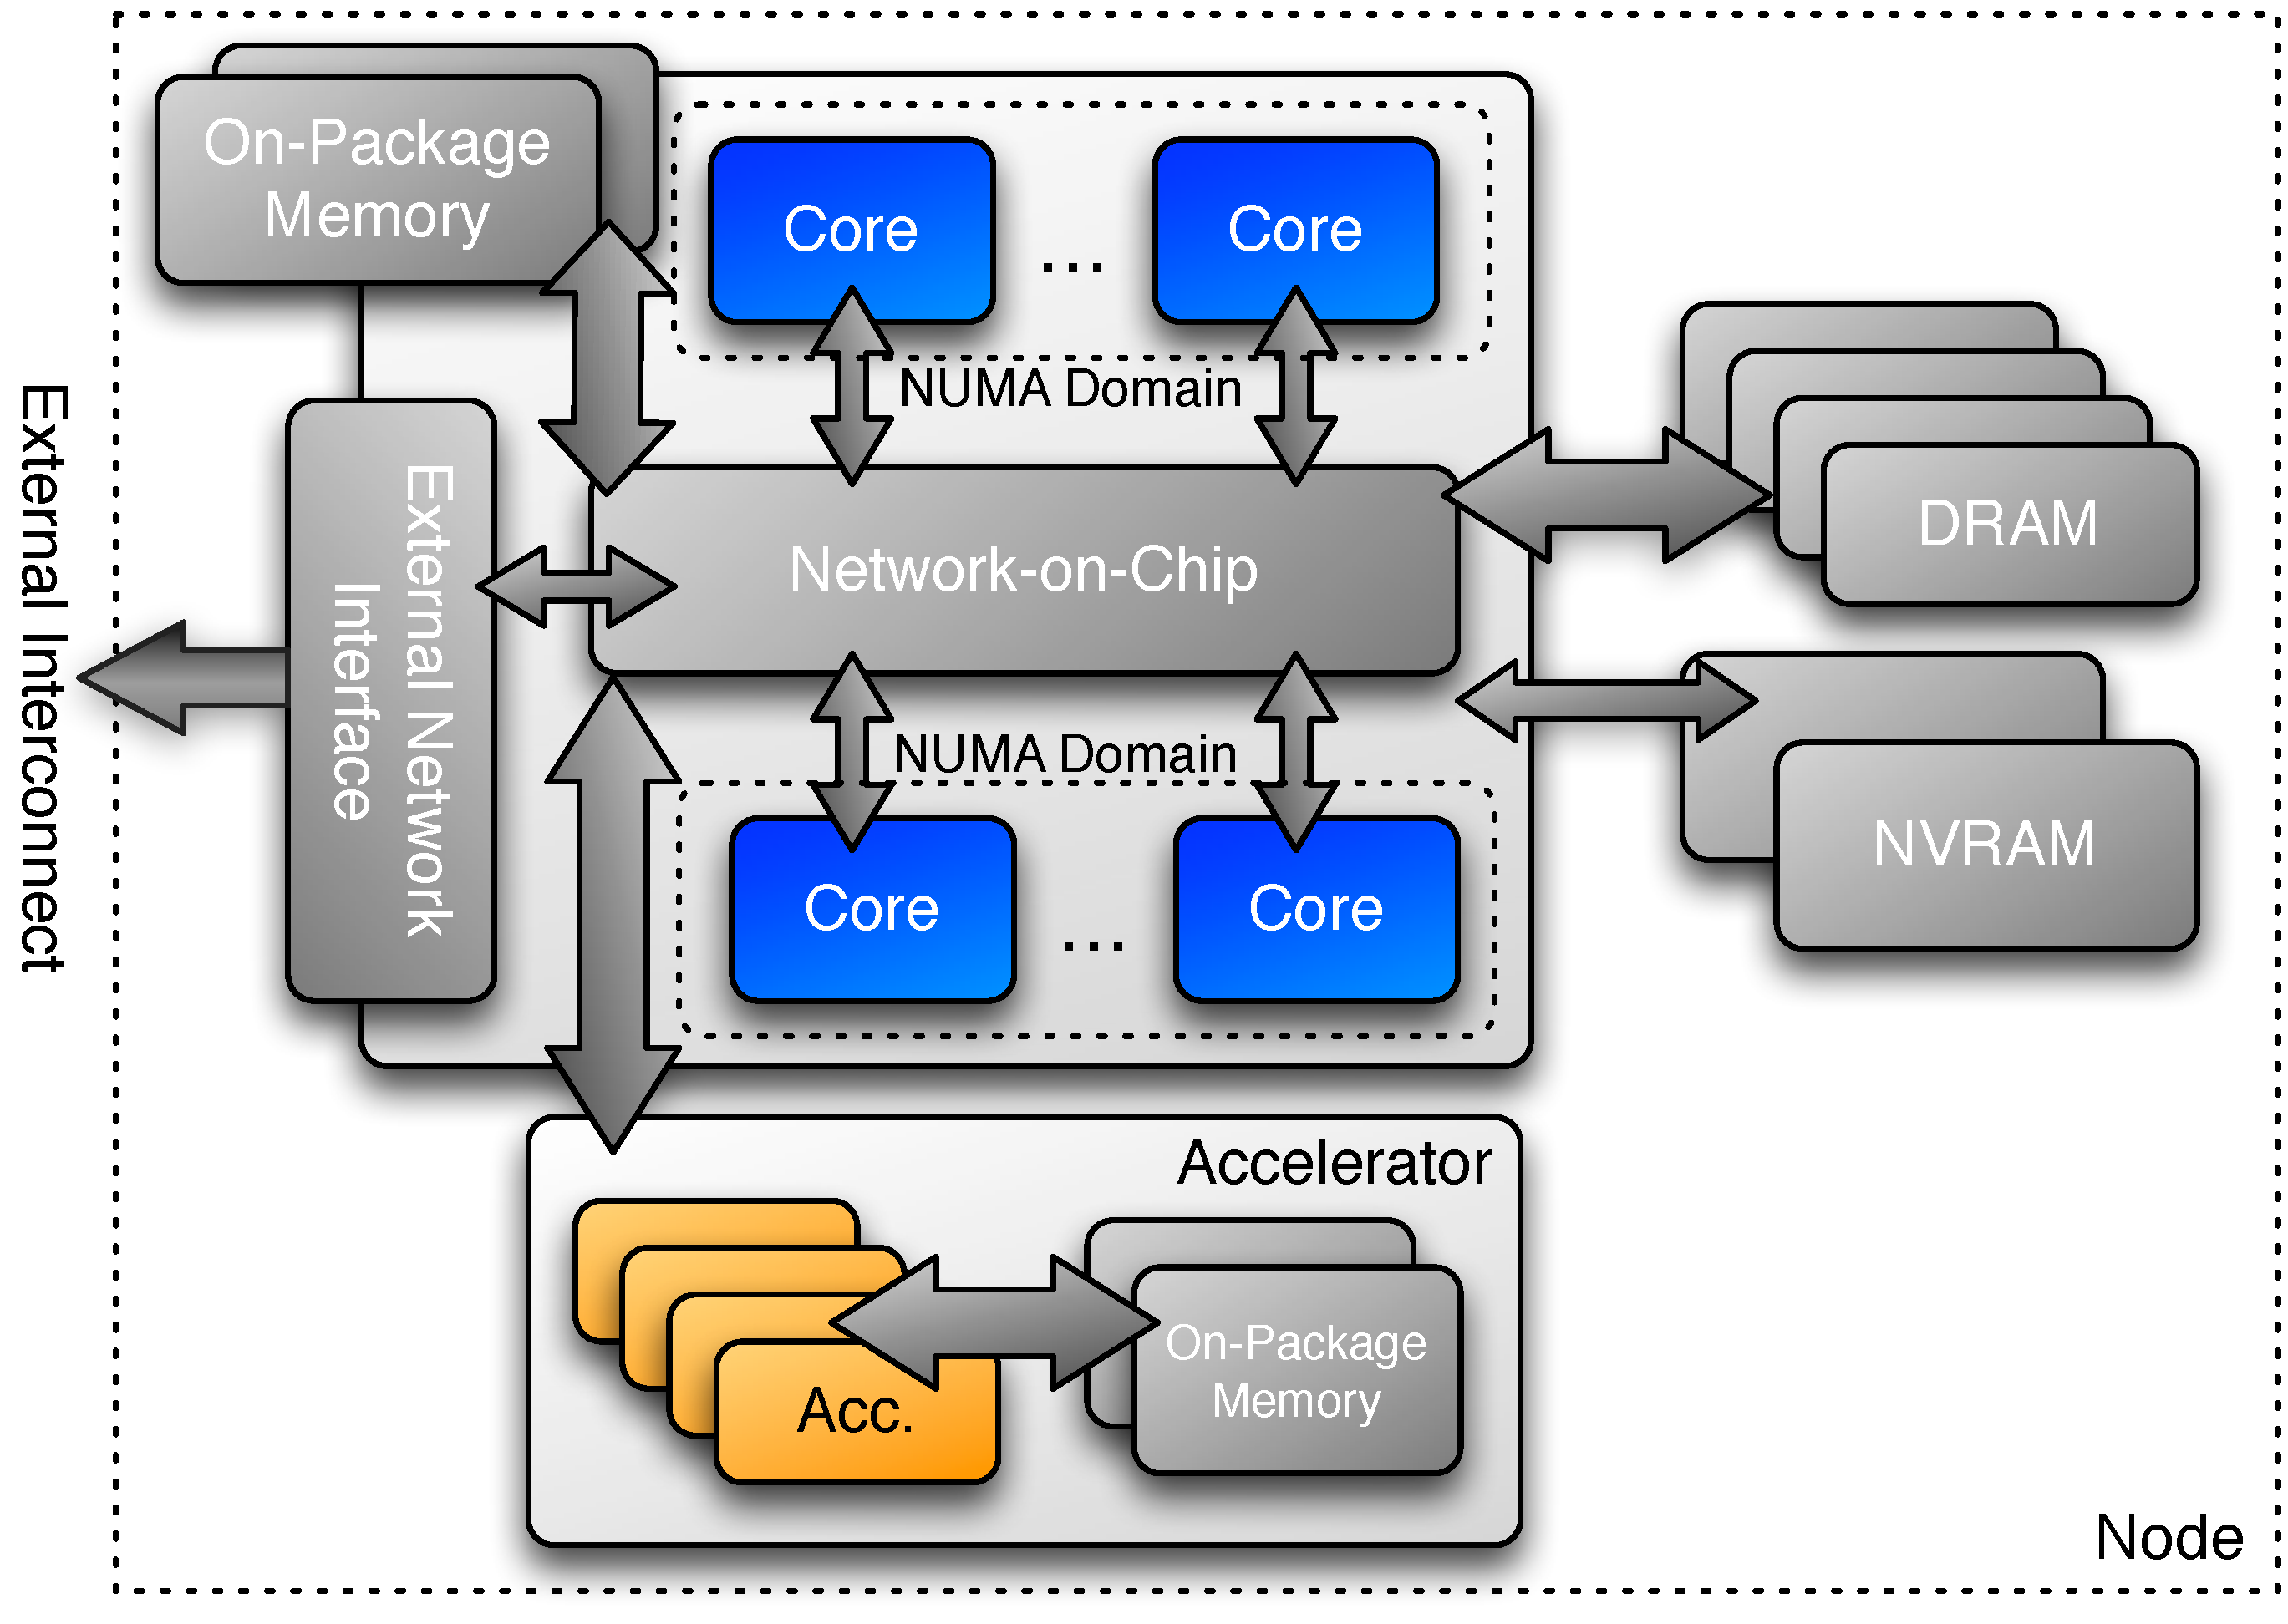
\includegraphics[width=0.70\textwidth]{figures/kokkos-execution-space}
  \end{center}

  \vspace{-12pt}

  {Execution spaces: \texttt{Serial, Threads, OpenMP, Cuda, HIP,} ... }

\end{frame}

%==========================================================================

\ifmedium
\begin{frame}[fragile]{Execution spaces (2)}

  \lstset{mathescape, escapeinside={<@}{@>},
          language=C,
          keywords={}}

  \begin{lstlisting}[linebackgroundcolor={
        \btLstHL{1-3}{darkred!20}
      }
    ]
  MPI_Reduce(...);
  FILE * file = fopen(...);
  runANormalFunction(...data...);
  \end{lstlisting}

  \vspace{-11pt}

  \begin{lstlisting}[linebackgroundcolor={
        \btLstHL{3-4}{bodyColor}
      }
    ]
  Kokkos::parallel_for("MyKernel", numberOfSomethings,
                       [=] (const int64_t somethingIndex) {
                         const double y = ...;
                         // do something interesting
                       }
                       );
  \end{lstlisting}

  \vspace{-5pt}

  \begin{textblock*}{0.5\textwidth}(0.08\textwidth,0.19\textheight)
    \rotatebox{90}{{\footnotesize {\color{darkred!80} Host}}}
  \end{textblock*}

  \begin{textblock*}{0.5\textwidth}(0.08\textwidth,0.315\textheight)
    \rotatebox{90}{{\footnotesize {\color{blue!80} Parallel}}}
  \end{textblock*}

  \pause

  \begin{itemize}
    \item<2->{Where will {\color{darkred!80}Host} code be run?  CPU?  GPU? \\
        \hspace{20pt}{$\Rightarrow$} Always in the \textbf{host process} \\
        \hspace{20pt} also known as \textbf{default host execution space}}
    \item<3->{Where will {\color{blue!80}Parallel} code be run?  CPU?  GPU? \\
      \hspace{20pt}{$\Rightarrow$} The \textbf{default execution space}}
    \item<4->{How do I \textbf{control} where the {\color{blue!80}Parallel} body is executed? \\
      \hspace{20pt}Changing the default execution space (\textit{at compilation}), \\
      \hspace{20pt}or specifying an execution space in the \textbf{policy}.}
  \end{itemize}

\end{frame}
\fi

%==========================================================================

\begin{frame}[fragile]{Execution spaces (3)}

  \textbf{\ul{Changing the parallel execution space:}}

  \vspace{3pt}

  \begin{code}[linebackgroundcolor={
        \btLstHL<1->{4}{bodyColor}
      },
      frame=single
    ]
@patternparallel_for@pattern("Label",
  @policyRangePolicy< @boldExecutionSpace@bold >(0,numberOfIntervals)@policy,
  [=] (const int64_t i) {
    /* ... body ... */
  });
  \end{code}

  \begin{code}[linebackgroundcolor={
        \btLstHL<1->{4}{bodyColor}
      },
      frame=single
    ]
@patternparallel_for@pattern("Label",
  @policynumberOfIntervals@policy, // => RangePolicy<>(0,numberOfIntervals)
  [=] (const int64_t i) {
    /* ... body ... */
  });
  \end{code}

  \begin{textblock*}{0.5\textwidth}(0.05\textwidth,0.465\textheight)
    \rotatebox{90}{\textbf{Default}}
  \end{textblock*}

  \begin{textblock*}{0.5\textwidth}(0.05\textwidth,0.23\textheight)
    \rotatebox{90}{\textbf{Custom}}
  \end{textblock*}

  \pause

  Requirements for enabling execution spaces:
  \vspace{-3pt}
  \begin{itemize}
    \item{Kokkos must be \textbf{compiled} with the execution spaces enabled.}
    \item{Execution spaces must be \textbf{initialized} (and \textbf{finalized}).}
    \item{\textbf{Functions} must be marked with a \textbf{macro} for non-CPU spaces.}
    \item{\textbf{Lambdas} must be marked with a \textbf{macro} for non-CPU spaces.}
  \end{itemize}

\end{frame}

%==========================================================================

\begin{frame}[fragile]{Execution spaces (5)}

  \textbf{\ul{Kokkos function and lambda portability annotation macros:}}

  \vspace{4pt}

  {Function annotation with \texttt{\footnotesize KOKKOS\_INLINE\_FUNCTION} macro}

  \begin{code}[keywords={}, frame=single, basicstyle=\tiny\ttfamily]
@graystruct ParallelFunctor {@gray
  KOKKOS_INLINE_FUNCTION
  @graydouble helperFunction(const int64_t s) const {...}@gray
  KOKKOS_INLINE_FUNCTION
  @grayvoid operator()(const int64_t index) const {
    helperFunction(index);
  }
}@gray
// Where kokkos defines:
#define KOKKOS_INLINE_FUNCTION inline                     // if CPU only
#define KOKKOS_INLINE_FUNCTION inline __device__ __host__ // if CPU + Cuda/HIP
  \end{code}

  \pause

  {Lambda annotation with \texttt{\footnotesize KOKKOS\_LAMBDA} macro}

  \begin{code}[keywords={}, frame=single, basicstyle=\tiny\ttfamily]
@grayKokkos::parallel_for("Label",numberOfIterations, @gray
  KOKKOS_LAMBDA@gray (const int64_t index) {...});@gray

// Where Kokkos defines:
#define KOKKOS_LAMBDA [=]                     // if CPU only
#define KOKKOS_LAMBDA [=] __device__ __host__ // if CPU + Cuda/HIP
  \end{code}

  These macros are \emph{already} defined by Kokkos.

  \vspace{-10pt}

\end{frame}

%==========================================================================

\ifmedium
\begin{frame}[fragile]{Memory Space Motivation}

  \ul{\textbf{Memory space motivating example:} summing an array}

  \begin{code}[linebackgroundcolor={
        \btLstHL<3-4>{3,10}{red!20}
      },
      keywords={}]
View<double*> data("data", size);
for (int64_t i = 0; i < size; ++i) {
  data(i) = ...read from file...
}

double sum = 0;
Kokkos::parallel_reduce("Label",
  RangePolicy<SomeExampleExecutionSpace>(0, size),
  KOKKOS_LAMBDA (const int64_t index, double & valueToUpdate) {
    valueToUpdate += data(index);
  },
  sum);
  \end{code}

  \pause
  \vspace{10pt}

  Question: Where is the data stored? GPU memory?  CPU memory?  Both?

  \pause
  \pause
  \vspace{10pt}

  \hspace{20pt}{\Large $\Rightarrow$ \textbf{Memory Spaces}}

\end{frame}
\fi

%==========================================================================

\begin{frame}[fragile]{Memory spaces (0)}

  \begin{center}
  \textbf{Memory space}: \\
     explicitly-manageable memory resource  \\
     (i.e., ``place to put data'')
  \end{center}

  \vspace{-20pt}

  \begin{center}
    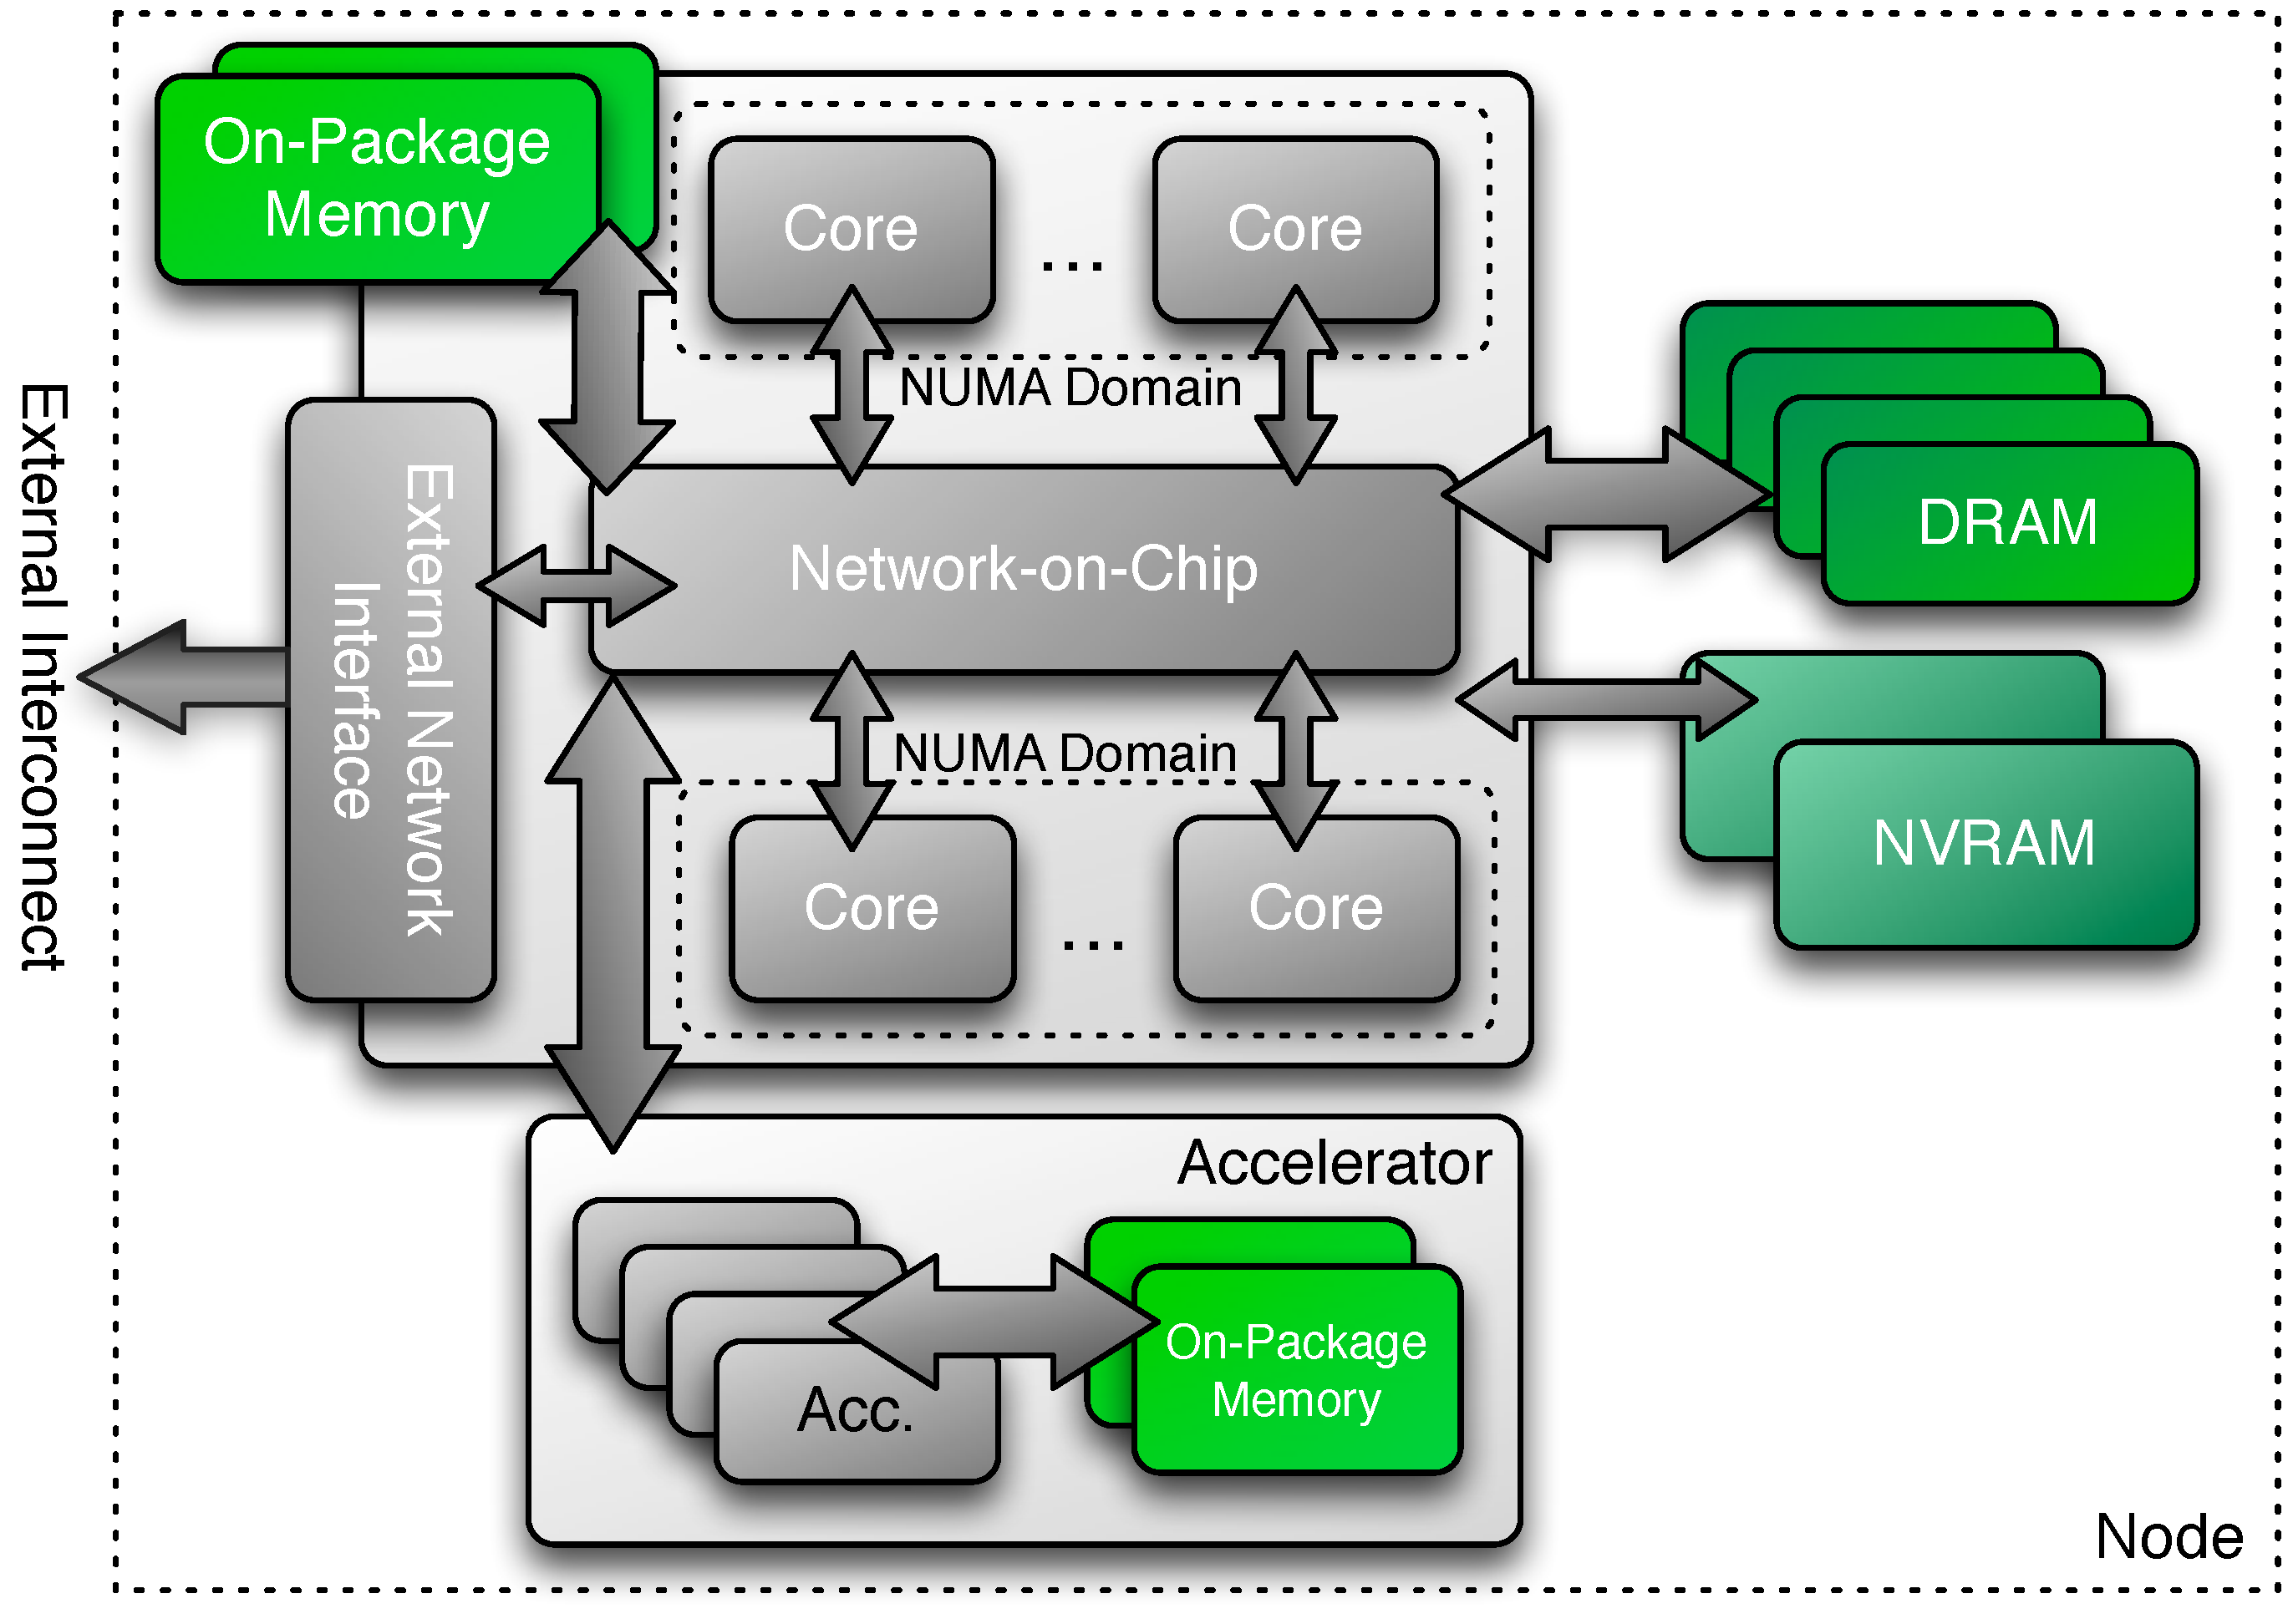
\includegraphics[width=0.75\textwidth]{figures/kokkos-memory-space}
  \end{center}

\end{frame}

%==========================================================================

\begin{frame}[fragile]{Memory spaces (1)}

  \begin{block}{Important concept: Memory spaces}
    Every view stores its data in a \textbf{memory space} set at compile time.
  \end{block}

  \vspace{10pt}

  \begin{itemize}
  \item<2->{\texttt{View<double***,}{\textit{Memory}\textbf{Space}}\texttt{> data(...);}}
  \item<3->{Available \textbf{memory spaces}: \\
            \hspace{20pt}\texttt{HostSpace, CudaSpace, CudaUVMSpace, ...} more} \\
            \hspace{20pt}Portable: \texttt{SharedSpace, SharedHostPinnedSpace}
  \item<4->{Each \textbf{execution space} has a default memory space, which is used if \textbf{Space} provided is actually an execution space}
  \item<5->{If no \texttt{Space} is provided, the view's data resides in the \textbf{default memory space} of the \textbf{default execution space}.}
  \end{itemize}

  \begin{uncoverenv}<6->
  \begin{code}[keywords={View,DefaultExecutionSpace,memory_space}]
  // Equivalent:
  View<double*> a("A",N);
  View<double*,DefaultExecutionSpace::memory_space> b("B",N);
  \end{code}
  \end{uncoverenv}
\end{frame}

%==========================================================================

\begin{frame}[fragile]{Memory spaces (2)}

  \ul{\textbf{Example: HostSpace}}

  \vspace{-3pt}

  \begin{code}[keywords={}]
View<double**, @boldHostSpace@bold> hostView(...constructor arguments...);
  \end{code}

  \vspace{-18pt}

  \begin{center}
    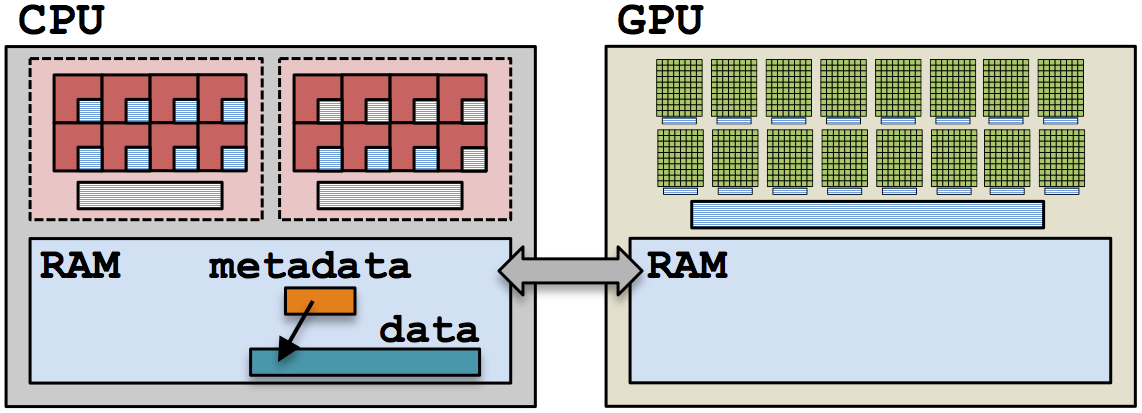
\includegraphics[width=0.70\textwidth]{figures/MemorySpaceExamples_hostSpace}
  \end{center}

  \vspace{-10pt}
  \pause

  \ul{\textbf{Example: CudaSpace}}

  \vspace{-3pt}

  \begin{code}[keywords={}]
View<double**, @boldCudaSpace@bold> view(...constructor arguments...);
  \end{code}

  \vspace{-18pt}

  \begin{center}
    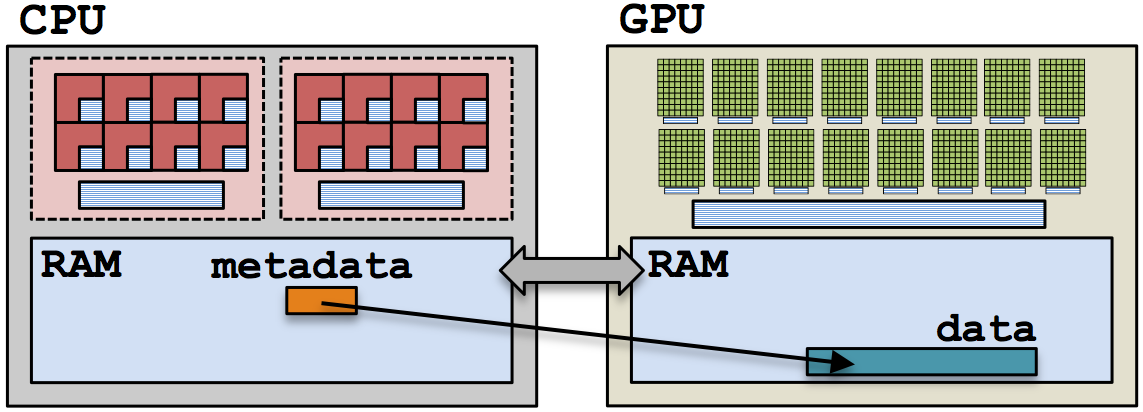
\includegraphics[width=0.70\textwidth]{figures/MemorySpaceExamples_cudaSpace}
  \end{center}

  \vspace{-10pt}

\end{frame}

%==========================================================================

\ifmedium
\begin{frame}[fragile]{Execution and Memory spaces (0)}

  \ul{\textbf{Anatomy of a kernel launch:}}

  \vspace{-10pt}

  \begin{columns}[t,onlytextwidth]

    \column{.6\textwidth}

      \begin{enumerate}
        \item{User declares views, allocating.}
        \item{User instantiates a functor with views.}
        \item{User launches \texttt{parallel\_something}:}
        \begin{itemize}
          \item{Functor is copied to the device.}
          \item{Kernel is run.}
          \item{Copy of functor on the device is released.}
        \end{itemize}
      \end{enumerate}

    \column{.40\textwidth}

      \vspace{10pt}

      \begin{code}[keywords={}]
#define KL KOKKOS_LAMBDA
View<int*, Cuda> @darkgreendev@darkgreen(...);
parallel_for("Label",N,
  KL (int i) {
    @darkgreendev@darkgreen(i) = ...;
  });
      \end{code}

      \vspace{20pt}

  \end{columns}

  \vspace{20pt}

  Note: \textbf{no deep copies} of array data are performed; \\
    \hspace{30pt}\emph{views are like pointers}.

\end{frame}
\fi

%==========================================================================

\ifmedium
\begin{frame}[fragile]{Execution and Memory spaces (1)}

  \begin{columns}[t,onlytextwidth]
    \column{.40\textwidth}

    \vspace{15pt}

    \ul{\textbf{Example: one view}}

    \vspace{5pt}

    \begin{code}[keywords={}]
#define KL KOKKOS_LAMBDA
View<int*, Cuda> @darkgreendev@darkgreen;
parallel_for("Label",N,
  KL (int i) {
    @darkgreendev@darkgreen(i) = ...;
  });
    \end{code}

    \column{.60\textwidth}

      \begin{center}
        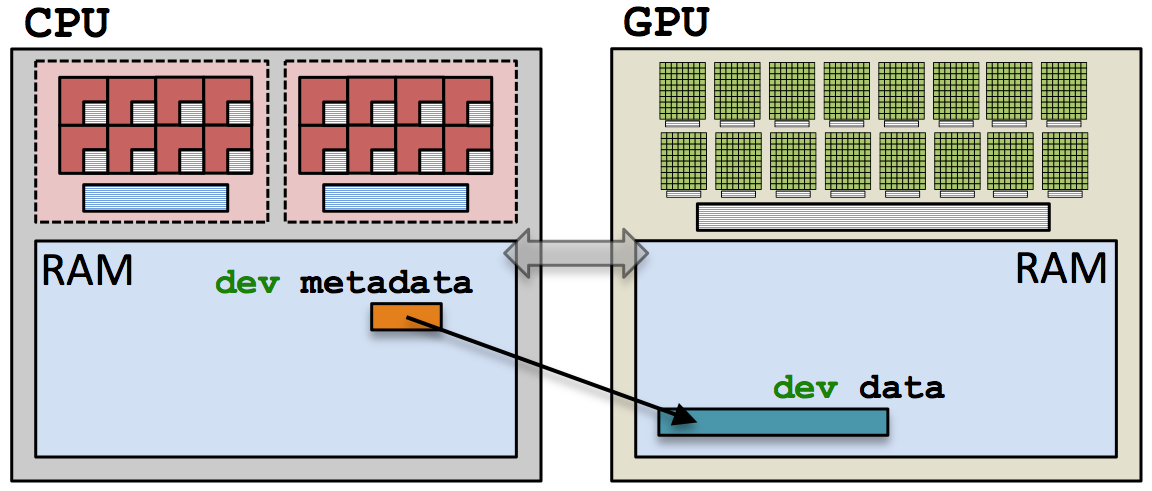
\includegraphics[width=1.00\textwidth]{figures/MemorySpaceExamples_cuda_0}
      \end{center}
      \begin{center}
        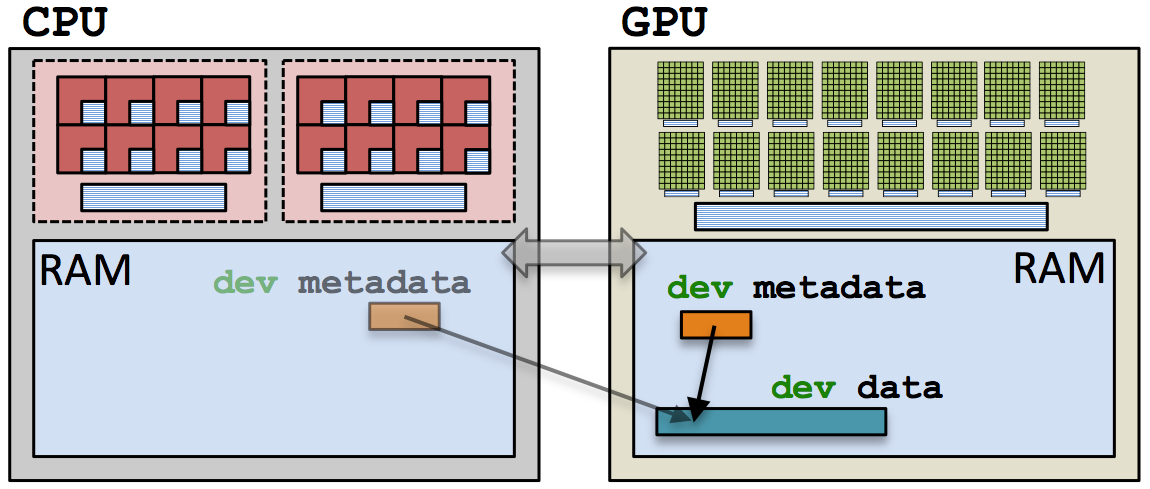
\includegraphics[width=1.00\textwidth]{figures/MemorySpaceExamples_cuda_1}
      \end{center}

  \end{columns}

\end{frame}
\fi

%==========================================================================

\ifmedium
\begin{frame}[fragile]{Execution and Memory spaces (2)}

  \begin{columns}[t,onlytextwidth]
    \column{.40\textwidth}

    \vspace{15pt}

    \ul{\textbf{Example: two views}}

    \vspace{5pt}

    \begin{code}[linebackgroundcolor={
          \btLstHL<2>{7}{red!20}
        },
        keywords={}]
#define KL KOKKOS_LAMBDA
View<int*, Cuda> @darkgreendev@darkgreen;
View<int*, Host> @bluehost@blue;
parallel_for("Label",N,
  KL (int i) {
    @darkgreendev@darkgreen(i)  = ...;
    @bluehost@blue(i) = ...;
  });
    \end{code}

    \column{.60\textwidth}

      \begin{center}
        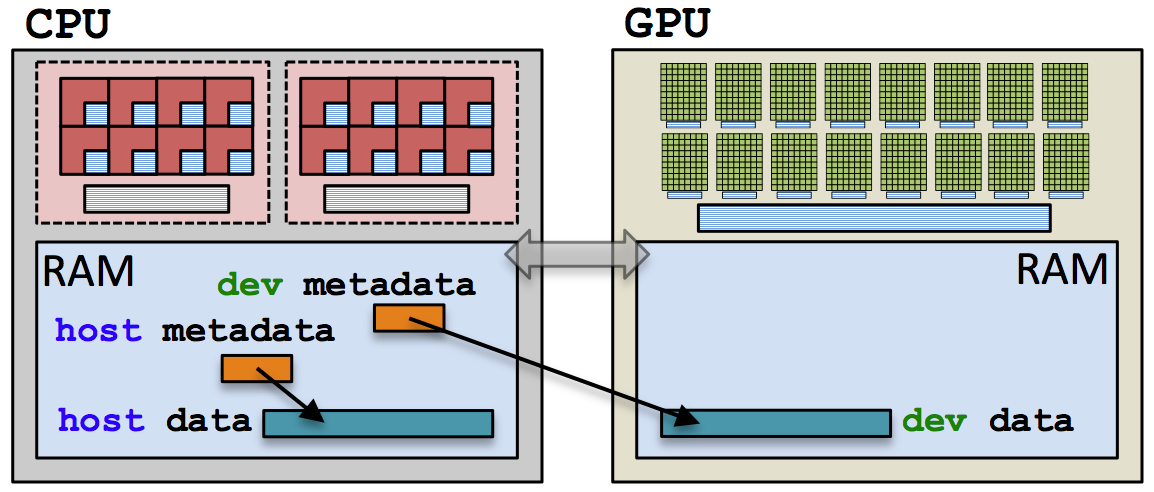
\includegraphics[width=1.00\textwidth]{figures/MemorySpaceExamples_hostCuda_0}
      \end{center}
      \begin{center}
        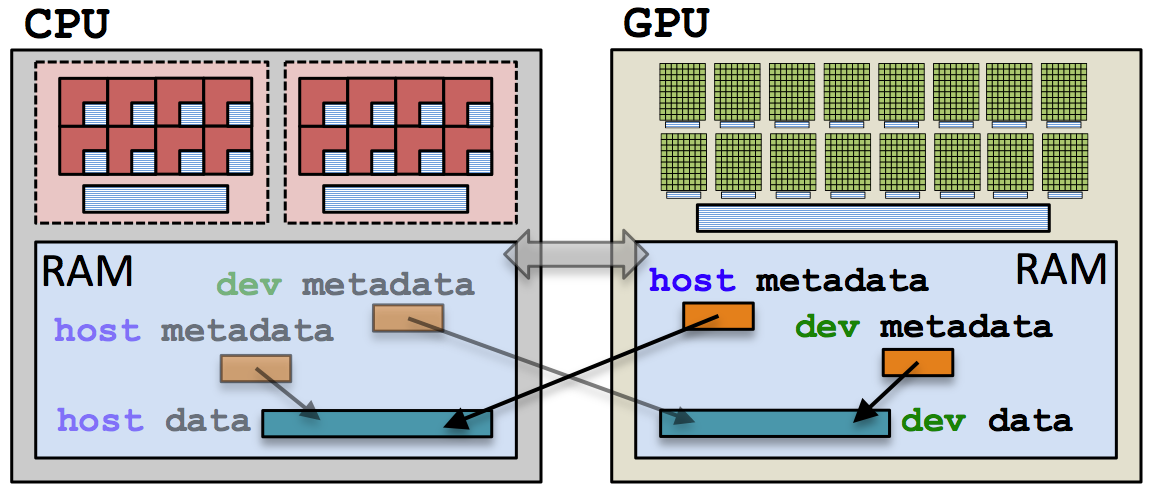
\includegraphics[width=1.00\textwidth]{figures/MemorySpaceExamples_hostCuda_1}
      \end{center}

  \end{columns}

\end{frame}
\fi

%==========================================================================

\begin{frame}[fragile]{Execution and Memory spaces (3)}

  \ul{\textbf{Example (redux): summing an array with the GPU}}

  \vspace{7pt}

  \hspace{10pt}(failed) Attempt 1: \texttt{View} lives in \texttt{CudaSpace}

  \vspace{3pt}

  \begin{code}[linebackgroundcolor={
        \btLstHL<2->{3}{red!20}
      },
      keywords={}]
View<double*, @boldCudaSpace@bold> array("array", size);
@grayfor (int64_t i = 0; i < size; ++i) {@gray
  array(i) = ...read from file...
@gray}@gray

@graydouble sum = 0;@gray
@grayKokkos::parallel_reduce("Label",@gray
  RangePolicy< @boldCuda@bold>(0, size),
  @grayKOKKOS_LAMBDA (const int64_t index, double & valueToUpdate) {@gray
    valueToUpdate += array(index);
  @gray},@gray
  @graysum);@gray
  \end{code}

  \vspace{11pt}

  \begin{textblock*}{0.5\textwidth}(0.94\textwidth,0.382\textheight)
    \only<2->{\texttt{fault}}
  \end{textblock*}

  \vspace{26pt}

\end{frame}

%==========================================================================

\begin{frame}[fragile]{Execution and Memory spaces (4)}

  \ul{\textbf{Example (redux): summing an array with the GPU}}

  \vspace{7pt}

  \hspace{10pt}(failed) Attempt 2: \texttt{View} lives in \texttt{HostSpace}

  \vspace{3pt}

  \begin{code}[linebackgroundcolor={
        \btLstHL<2-3>{10}{red!20}
      },
      keywords={}]
View<double*, @boldHostSpace@bold> array("array", size);
@grayfor (int64_t i = 0; i < size; ++i) {@gray
  array(i) = ...read from file...
@gray}@gray

@graydouble sum = 0;@gray
@grayKokkos::parallel_reduce("Label",@gray
  RangePolicy< @boldCuda@bold>(0, size),
  @grayKOKKOS_LAMBDA (const int64_t index, double & valueToUpdate) {@gray
    valueToUpdate += array(index);
  @gray},@gray
  @graysum);@gray
  \end{code}

  \vspace{3pt}

  \begin{textblock*}{0.5\textwidth}(0.82\textwidth,0.630\textheight)
    \only<2->{\texttt{illegal access}}
  \end{textblock*}

  \pause
  \pause
  \begin{columns}[t,onlytextwidth]
    \column{.35\textwidth}
      What's the solution?
    \column{.65\textwidth}
      \vspace{-25pt}
      \begin{itemize}
        \item{\texttt{SharedSpace}}
        \item{\texttt{SharedHostPinnedSpace} (skipping)}
        \item{Mirroring}
      \end{itemize}
  \end{columns}

\end{frame}

%==========================================================================

\ifmedium
\begin{frame}[fragile]{Execution and Memory spaces (5)}

  \vspace{-30pt}

  \begin{columns}[t,onlytextwidth]
    \column{.40\textwidth}

    \vspace{15pt}

    \ul{\texttt{SharedSpace}}

    \vspace{5pt}

    \begin{code}[keywords={}]
#define KL KOKKOS_LAMBDA
View<double*,
     @boldSharedSpace@bold> @darkgreenarray@darkgreen;
@darkgreenarray@darkgreen = ...from file...
double sum = 0;
parallel_reduce("Label", N,
  KL (int i, double & d) {
    d += @darkgreenarray@darkgreen(i);
  },
  sum);
    \end{code}

    \vspace{5pt}

    %{\color{red}Warning:} \\ \hspace{10pt}Performance penalty

    \column{.55\textwidth}

      \begin{center}
        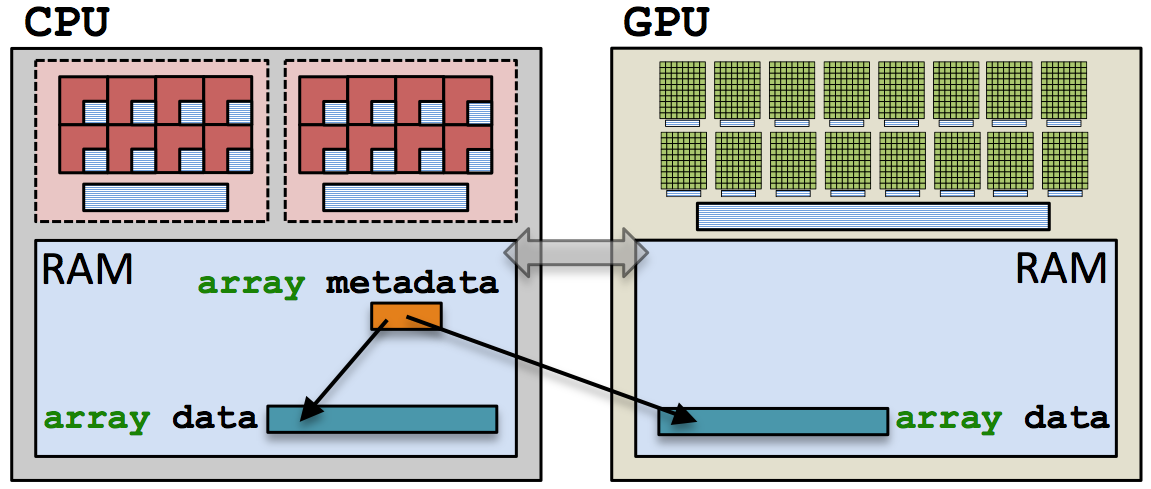
\includegraphics[width=0.95\textwidth]{figures/MemorySpaceExamples_uvm_0}
      \end{center}
      \begin{center}
        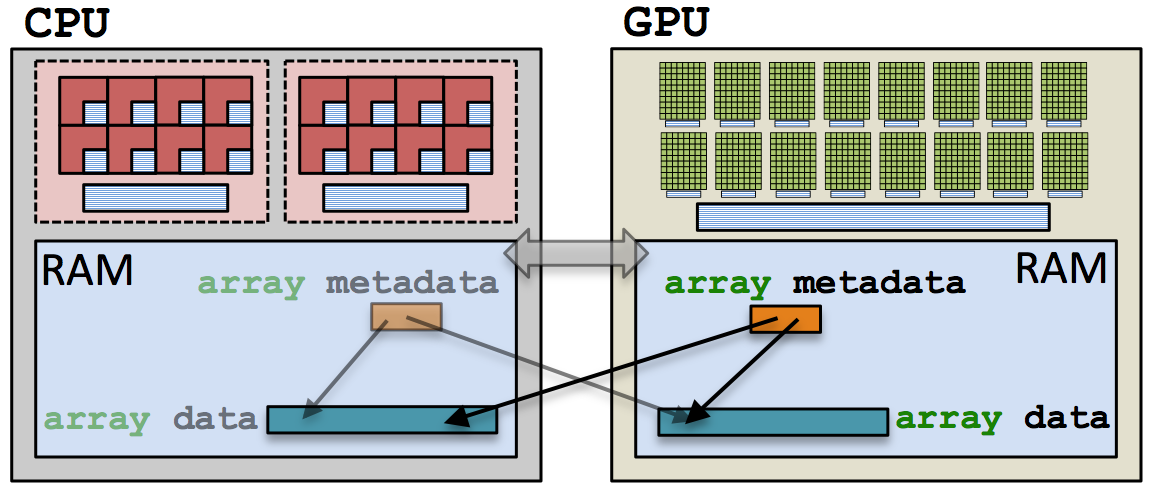
\includegraphics[width=0.95\textwidth]{figures/MemorySpaceExamples_uvm_1}
      \end{center}

  \end{columns}

  \vspace{10pt}

  Cuda runtime automatically handles data movement,
  \\ at a \textbf{performance hit}.

\end{frame}
\fi

\begin{comment}
\begin{frame}[fragile]{Exercise: CG-Solve}

  \textbf{Exercise}: Find $x$ in $b = A * x$

  Getting set up in your home directory:
  \begin{code}
    mkdir Kokkos
    cd Kokkos
    git clone https://github.com/kokkos/kokkos
    git clone https://github.com/kokkos/kokkos-tutorials
  \end{code}

  \vspace{5pt}
  Find the exercise in the kokkos-turoials/Exercises/cg-solve folder.


  \vspace{5pt}
  The Begin subdirectory contains the code. Only cg\_solve.cpp needs modifications.

  \vspace{5pt}
  Look for EXERCISE comments to find places to modify.

\end{frame}

%==========================================================================

\begin{frame}[fragile]{Exercise \#1: include, initialize, finalize Kokkos}

  The \textbf{first step} in using Kokkos is to include, initialize, and finalize:

  \begin{code}
#include <Kokkos_Core.hpp>
int main(int argc, char* argv[]) {
  /* ... do any necessary setup (e.g., initialize MPI) ... */
  Kokkos::initialize(argc, argv);
  {
  /* ... do computations ... */
  }
  Kokkos::finalize();
  return 0;
}
  \end{code}

  \vspace{7pt}

  (Optional) Command-line arguments or environment variables:

  \vspace{3pt}

	\begin{tabular}{| p{0.5\textwidth} | p{0.5\textwidth} |}
    \hline
	  \texttt{--kokkos-threads=INT} or \texttt{KOKKOS\_NUM\_THREADS} & total number of threads \\
    \hline
	  \texttt{--kokkos-device-id=INT} or \texttt{KOKKOS\_DEVICE\_ID} & device (GPU) ID to use \\
    \hline
  \end{tabular}

\end{frame}

%==========================================================================



\begin{frame}[fragile]{Exercise: Compiling}

\ul{\textbf{Compiling for CPU}}

\vspace{-3pt}
  \begin{small}
  \begin{code}
    cmake -B build_openmp -D Kokkos_ENABLE_OPENMP=ON
    cmake --build build_openmp -j
  \end{code}
  Optional: configure with \texttt{Kokkos\_ARCH\_NATIVE=ON} or specify explicitly the target architecture
  \end{small}

%  \hspace{10pt} {\tiny \url{https://github.com/kokkos/kokkos/wiki/Compiling#table-43-architecture-variables}}

\ul{\textbf{Running on CPU} with OpenMP back-end}

\vspace{-3pt}
  \begin{small}
  \begin{code}
  # Set OpenMP affinity
  export OMP_NUM_THREADS=8
  export OMP_PROC_BIND=spread OMP_PLACES=threads
  # Print example command line options:
  ./cg\_solve.exe -h
  # Run with defaults on CPU
  ./cg\_solve.exe
  # Run larger problem
  ./cg\_solve.exe 200 200
  \end{code}
  \end{small}

\ul{\textbf{Things to try:}}
  \begin{small}
  \begin{itemize}
  \itemsep0em
  \item Vary number of threads
  \item Vary problem size
  \item Compare Serial backend performance to unmodified code
  \end{itemize}
  \end{small}
\end{frame}

\begin{frame}[fragile]{Exercise: Compiling}

\ul{\textbf{Compiling for GPU}}

\vspace{-3pt}
  \begin{small}
  \begin{code}
    cmake -B build_openmp -D Kokkos_ENABLE_OPENMP=ON
    cmake --build build_openmp -j
  \end{code}
  Optional: configure with \texttt{Kokkos\_ARCH\_NATIVE=ON} or specify explicitly the target architecture
  \end{small}

%  \hspace{10pt} {\tiny \url{https://github.com/kokkos/kokkos/wiki/Compiling#table-43-architecture-variables}}

\ul{\textbf{Things to try:}}
  \begin{small}
  \begin{itemize}
  \itemsep0em
  \item Vary number of iterations
  \item Vary problem size
  \item Compare performance to CPU runs? What is the ratio compared to expected bandwidth ratio?
  \end{itemize}
  \end{small}
\end{frame}
\end{comment}

%==========================================================================
%==========================================================================

\begin{frame}[fragile]{Views, Spaces, and Mirrors}

  \begin{block}{Important concept: Mirrors}
    Mirrors are views of equivalent arrays residing in possibly different memory spaces.
  \end{block}

  \vspace{3pt}
  \pause

  \ul{\textbf{Mirroring schematic}}

  \vspace{-3pt}

  \begin{code}[keywords={view_type}]
Kokkos::View<double**, @boldSpace@bold> @darkgreenview@darkgreen(...);
auto @darkredhostView@darkred = @boldKokkos::create_mirror_view@bold(@darkgreenview@darkgreen);
  \end{code}

  \vspace{-8pt}

  \begin{center}
    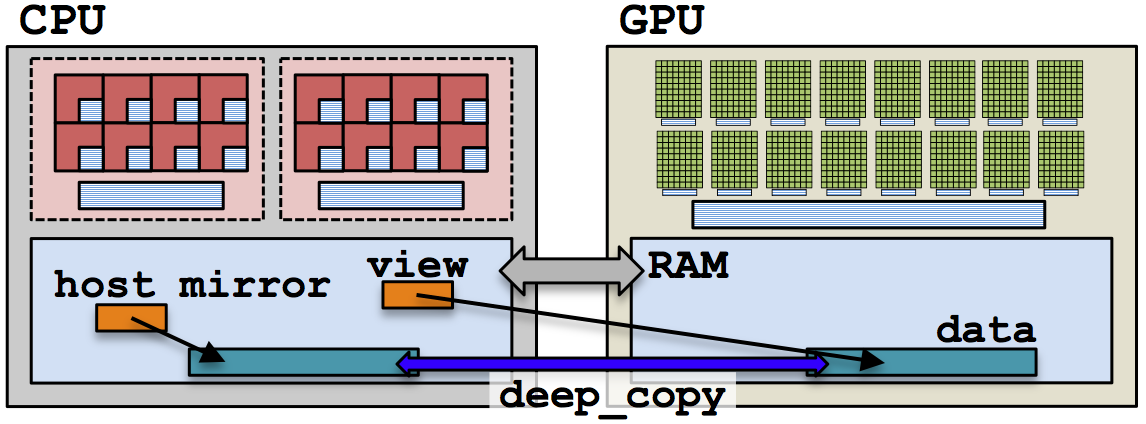
\includegraphics[width=0.70\textwidth]{figures/MemorySpaceExamples_mirrors}
  \end{center}

  \vspace{-10pt}

\end{frame}

%==========================================================================

\begin{frame}[fragile]{Mirroring pattern}

  \begin{enumerate}
    \item<+->{\textbf{Create} a {\color{darkgreen}\texttt{view}}'s array in some memory space. \\

      \vspace{-5pt}
      \begin{code}[keywords={view_type}]
  Kokkos::View<double*, @boldSpace@bold> @darkgreenview@darkgreen(...);
      \end{code}
      \vspace{-4pt}

  }
    \item<+->{\textbf{Create} {\color{darkred}\texttt{hostView}}, a \textit{mirror} of the {\color{darkgreen}\texttt{view}}'s array residing in the host memory space. \\

      \vspace{-5pt}
      \begin{code}[keywords={view_type}]
  auto @darkredhostView@darkred = @boldKokkos::create_mirror_view@bold(@darkgreenview@darkgreen);
      \end{code}
      \vspace{-4pt}

  }
    \item<+->{\textbf{Populate} {\color{darkred}\texttt{hostView}} on the host (from file, etc.).}
    \item<+->{\textbf{Deep copy} {\color{darkred}\texttt{hostView}}'s array to {\color{darkgreen}\texttt{view}}'s array. \\

      \vspace{-5pt}
      \begin{code}[keywords={}]
  Kokkos::@bolddeep_copy@bold(@darkgreenview@darkgreen, @darkredhostView@darkred);
      \end{code}
      \vspace{-4pt}

  }
    \item<+->{\textbf{Launch} a kernel processing the {\color{darkgreen}\texttt{view}}'s array. \\

      \vspace{-5pt}
      \begin{code}[keywords={}]
  Kokkos::parallel_for("Label",
    RangePolicy< @boldSpace@bold>(0, size),
    KOKKOS_LAMBDA (...) { use and change @darkgreenview@darkgreen });
      \end{code}
      \vspace{-4pt}

  }
    \item<+->{If needed, \textbf{deep copy} the {\color{darkgreen}\texttt{view}}'s updated array back to the {\color{darkred}\texttt{hostView}}'s array to write file, etc. \\

      \vspace{-5pt}
      \begin{code}[keywords={}]
  Kokkos::@bolddeep_copy@bold(@darkredhostView@darkred, @darkgreenview@darkgreen);
      \end{code}
      \vspace{-4pt}

  }
  \end{enumerate}

\end{frame}

%==========================================================================

\begin{frame}[fragile]{Mirrors of \texttt{View}s in \texttt{HostSpace}}

  What if the \texttt{View} is in \texttt{HostSpace} too?  Does it make a copy?

  \begin{code}[keywords={}]
Kokkos::View<double*, @boldSpace@bold> @darkgreenview@darkgreen("test", 10);
auto @darkredhostView@darkred = @boldKokkos::create_mirror_view@bold(@darkgreenview@darkgreen);
  \end{code}

  \begin{itemize}
    \item{\texttt{create\_mirror\_view} allocates data only if the host process cannot access {\color{darkgreen}view}'s data, otherwise {\color{darkred}hostView} references the same data.}
    \item{\texttt{create\_mirror} \textbf{always} allocates data.}
    \item{\texttt{create\_mirror\_view\_and\_copy} allocates data if necessary and also \textbf{copies} data.}
  \end{itemize}

  Reminder: Kokkos \emph{never} performs a \textbf{hidden deep copy}.

  \vspace{-5pt}

\end{frame}

%==========================================================================

\begin{frame}[fragile]{Exercise \#3: Flat Parallelism on the GPU, Views and Host Mirrors}

  \textbf{Details}:
  \begin{scriptsize}
  \begin{itemize}
\item Location: \ExerciseDirectory{03/Begin}
\item Add HostMirror Views and deep copy
\item Make sure you use the correct view in initialization and Kernel
\end{itemize}
  \end{scriptsize}

\begin{code}
  # Compile for CPU
  cmake -B build_openmp -DKokkos_ENABLE_OPENMP=ON
  cmake --build build_openmp
  # Run on CPU
  ./build_openmp/03_Exercise -S 26
  # Note the warnings, set appropriate environment variables
  # Compile for GPU
  cmake -B build_cuda -DKokkos_ENABLE_CUDA=ON
  cmake --build build_cuda
  # Run on GPU
  ./build_cuda/03_Exercise -S 26
\end{code}

  \ul{\textbf{Things to try:}}
  \begin{scriptsize}
  \begin{itemize}
  \item Vary problem size and number of rows (-S ...; -N ...)
  \item Change number of repeats (-nrepeat ...)
  \item Compare behavior of CPU vs GPU
  \end{itemize}
  \end{scriptsize}



\end{frame}

%==========================================================================

\begin{frame}[fragile]{View and Spaces Section Summary}

  \begin{itemize}
    \item{Data is stored in \texttt{Views} that are ``pointers'' to \textbf{multi-dimensional arrays} residing in \textbf{memory spaces}.}
    \item{\texttt{Views} \textbf{abstract away} platform-dependent allocation, (automatic) deallocation, and access.}
    \item{\textbf{Heterogeneous nodes} have one or more memory spaces.}
    \item{\textbf{Mirroring} is used for performant access to views in host and device memory.}
    \item{Heterogeneous nodes have one or more \textbf{execution spaces}.}
    \item{You \textbf{control where} parallel code is run by a template parameter on the execution policy, or by compile-time selection of the default execution space.}
  \end{itemize}

\end{frame}


\begin{frame}[fragile]

  {\huge Managing memory access patterns \\ for performance portability}

  \vspace{20pt}

  \textbf{Learning objectives:}
  \begin{itemize}
    \item{How the \texttt{View}'s \texttt{Layout} parameter controls data layout.}
    \item{How memory access patterns result from Kokkos mapping parallel work indices \textbf{and} layout of multidimensional array data}
    \item{Why memory access patterns and layouts have such a performance impact (caching and coalescing).}
    \item{See a concrete example of the performance of various memory configurations.}
  \end{itemize}

  \vspace{-20pt}

\end{frame}

%==========================================================================

\begin{frame}[fragile]{Example: inner product (0)}

  \begin{code}[keywords={}]
Kokkos::parallel_reduce("Label", 
  RangePolicy<ExecutionSpace>(0, N),
  KOKKOS_LAMBDA (const size_t row, double & valueToUpdate) {
    double thisRowsSum = 0;
    for (size_t entry = 0; entry < M; ++entry) {
      thisRowsSum += @blueA@blue(row, entry) * @darkgreenx@darkgreen(entry);
    }
    valueToUpdate += @darkredy@darkred(row) * thisRowsSum;
  }, @orangeresult@orange);
  \end{code}

  \vspace{-20pt}

  \begin{center}
    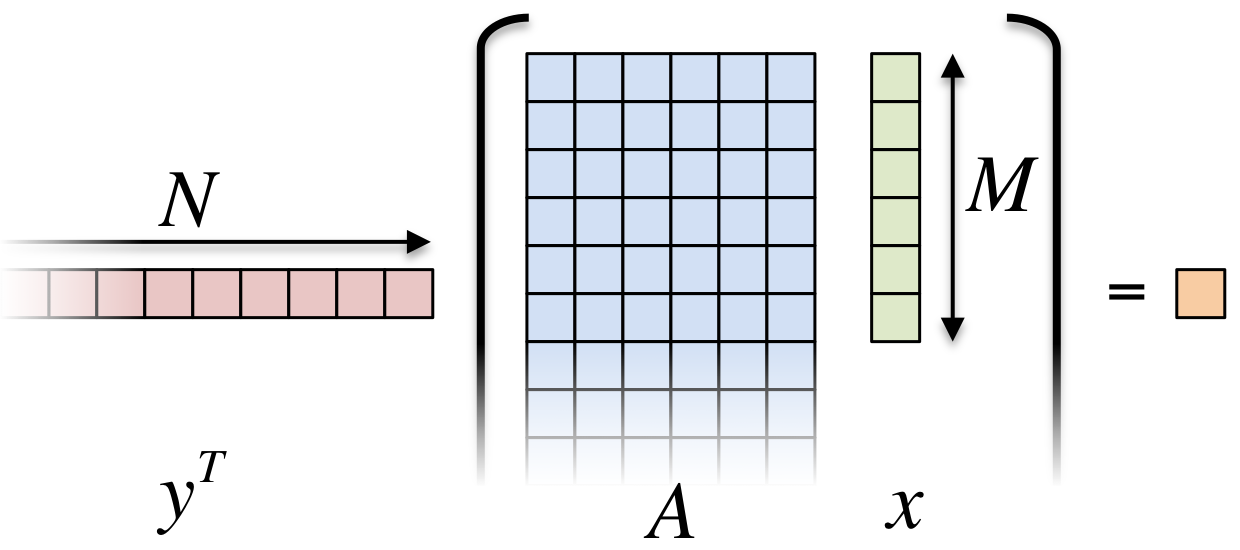
\includegraphics[width=0.8\textwidth]{figures/InnerProductExample_LayoutIntro}
  \end{center}

  \pause
  \vspace{-8pt}

 \textbf{Driving question:} How should {\color{blue}\texttt{A}} be laid out in memory?

  \vspace{8pt}

\end{frame}

%==========================================================================

\begin{frame}[fragile]{Example: inner product (1)}

  Layout is the mapping of multi-index to memory:

  \vspace{-10pt}

  \begin{columns}[t,onlytextwidth]
    \column{.40\textwidth}

      \vspace{20pt}

      \ul{\textbf{LayoutLeft}} \\
      \vspace{3pt}
      \hspace{10pt} in 2D, ``column-major''

      \vspace{50pt}

      \ul{\textbf{LayoutRight}} \\
      \vspace{3pt}
      \hspace{10pt} in 2D, ``row-major''
    \column{.60\textwidth}
      \begin{center}
        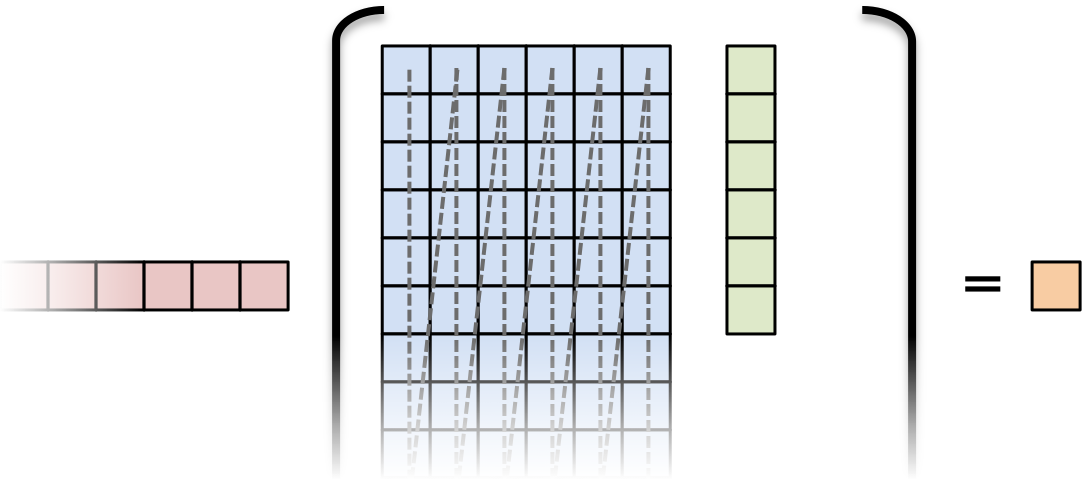
\includegraphics[width=1.00\textwidth]{figures/InnerProductExample_LayoutLeft}
        \\
        \vspace{10pt}
        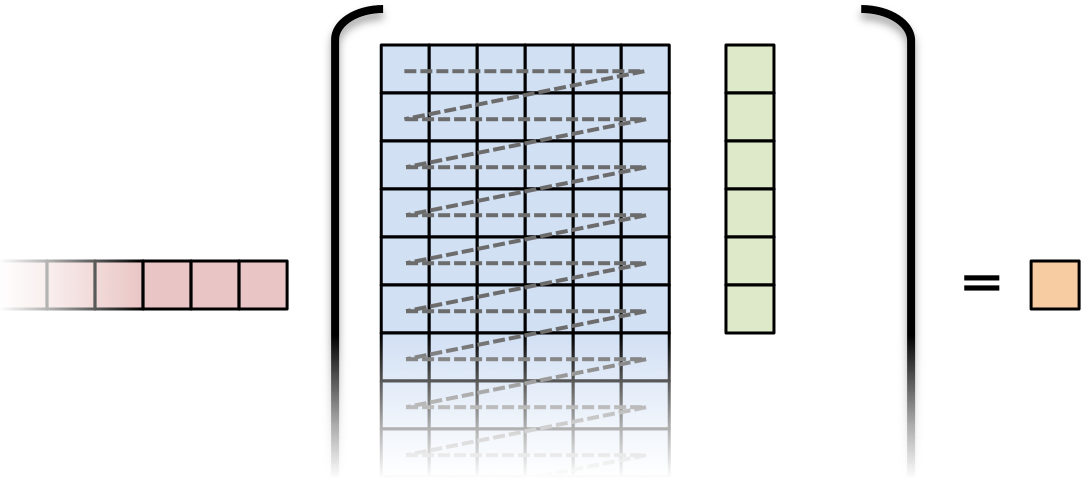
\includegraphics[width=1.00\textwidth]{figures/InnerProductExample_LayoutRight}
      \end{center}
  \end{columns}

\end{frame}

%==========================================================================

\begin{frame}[fragile]{Layout}

  \begin{block}{Important concept: Layout}
    Every \texttt{View} has a multidimensional array \texttt{Layout} set at compile-time.
  \end{block}

  \vspace{5pt}

  \begin{code}[frame=single, keywords={}]
View<double***, @boldLayout@bold, Space> name(...);
  \end{code}

  \pause
  \vspace{-5pt}

  \begin{itemize}
    \item{Most-common layouts are \texttt{LayoutLeft} and \texttt{LayoutRight}. \\
      \hspace{10pt} \texttt{LayoutLeft}: left-most index is stride 1.\\
      \hspace{10pt} \texttt{LayoutRight}: right-most index is stride 1.}
    \item{If no layout specified, default for that memory space is used. \\
      \hspace{10pt} \texttt{LayoutLeft} for \texttt{CudaSpace}, \texttt{LayoutRight} for \texttt{HostSpace}.}
    \item{Layouts are extensible: $\approx$ 50 lines}
    \item{Advanced layouts: \texttt{LayoutStride}, \texttt{LayoutTiled}, ...}
  \end{itemize}

  \vspace{-15pt}

\end{frame}

%==========================================================================

\begin{frame}[fragile]{Exercise \#4: Inner Product, Flat Parallelism}

  \textbf{Details}:
  \begin{small}
  \begin{itemize}
\item Location: \ExerciseDirectory{04/Begin}
\item Replace \texttt{``N''} in parallel dispatch with \texttt{RangePolicy<ExecSpace>}
\item Add \texttt{MemSpace} to all \texttt{Views} and \texttt{Layout} to \texttt{A}
\item Experiment with the combinations of \texttt{ExecSpace}, \texttt{Layout} to view performance
\end{itemize}
  \end{small}


\ul{\textbf{Things to try:}}
  \begin{small}
  \begin{itemize}
  \item Vary problem size and number of rows (-S ...; -N ...)
  \item Change number of repeats (-nrepeat ...)
  \item Compare behavior of CPU vs GPU
  \item Compare using UVM vs not using UVM on GPUs
  \item Check what happens if \texttt{MemSpace} and \texttt{ExecSpace} do not match.
  \end{itemize}
  \end{small}
\end{frame}

%==========================================================================

\begin{frame}[fragile]{Exercise \#4: Inner Product, Flat Parallelism}


  \vspace{-10pt}

    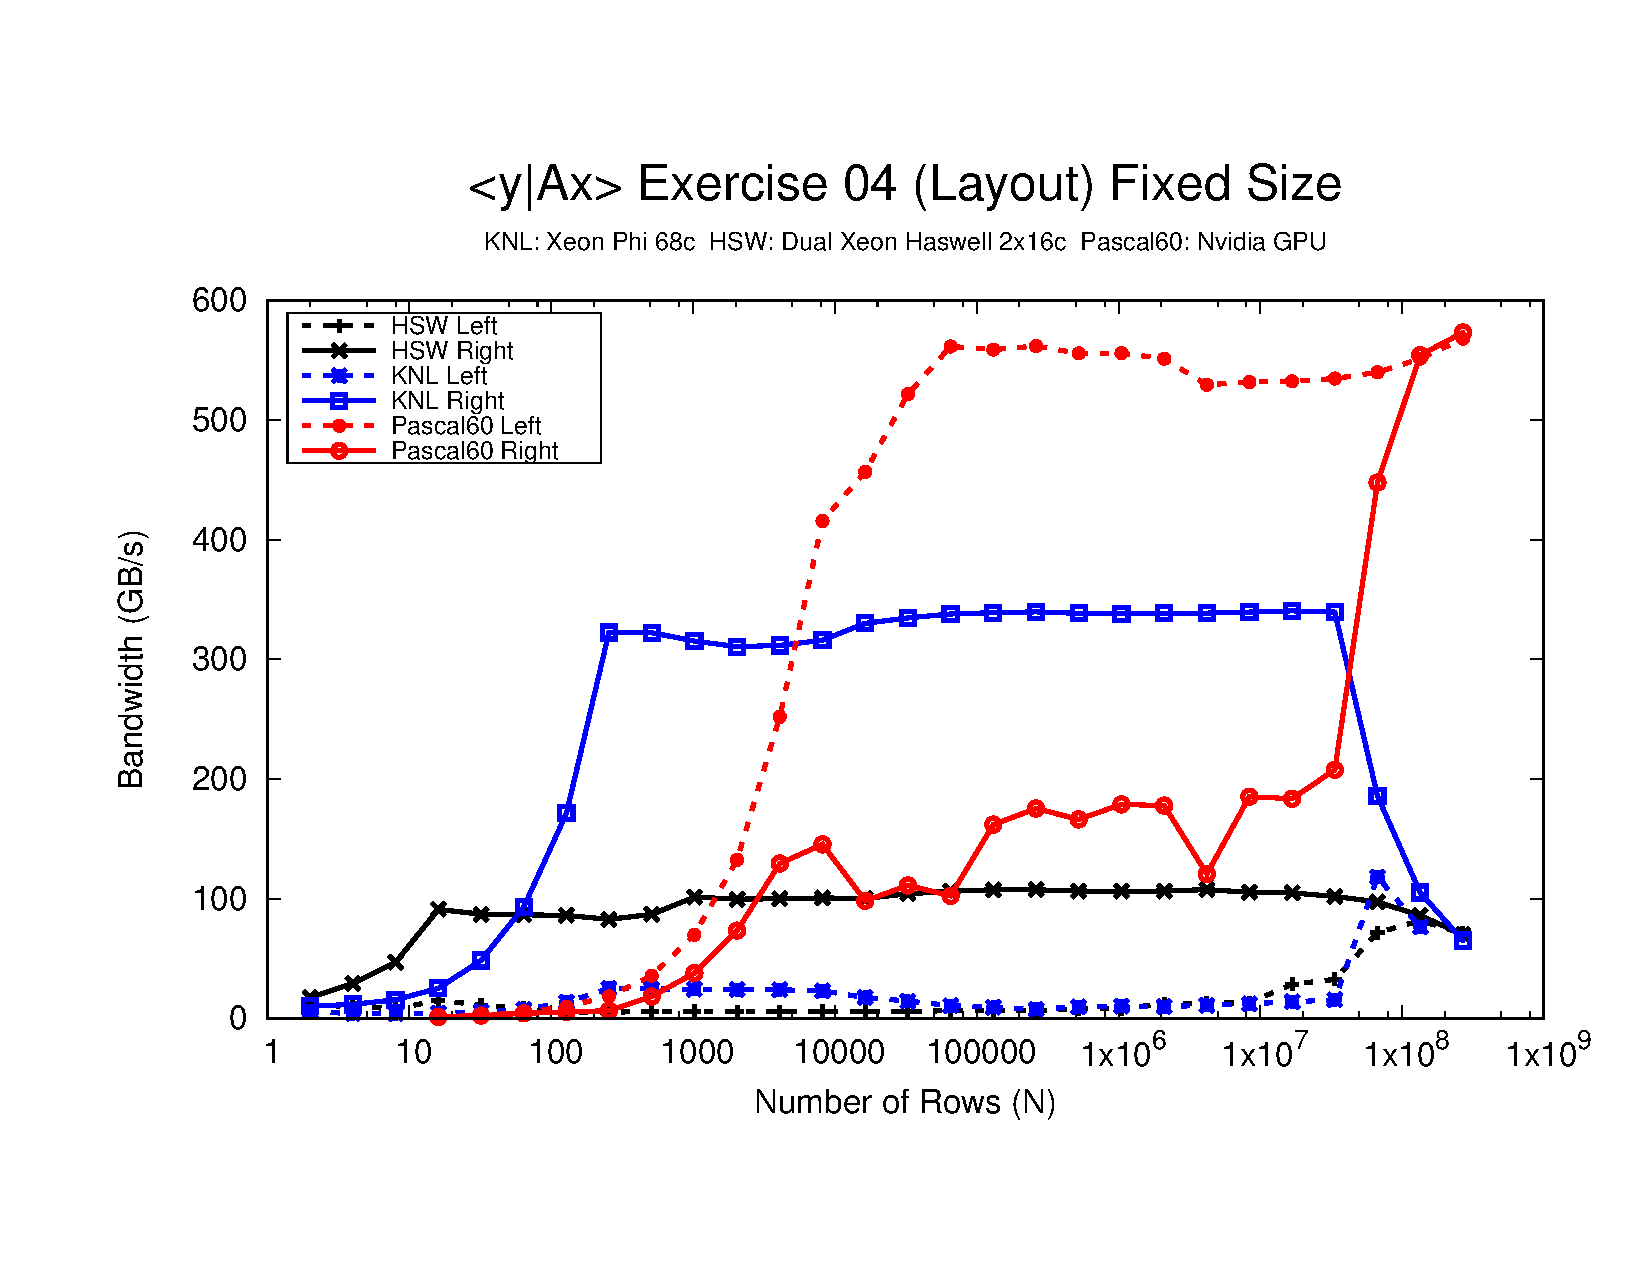
\includegraphics[viewport=1.25in 3.0in 10in 6in, width=0.95\textwidth]{figures/Exercise04-Performance.pdf}

  \vspace{-15pt}

  \begin{textblock*}{0.5\textwidth}(0.97\textwidth,0.50\textheight)
    \textbf{\LARGE Why?}
  \end{textblock*}

\end{frame}

%==========================================================================

\begin{frame}[fragile]{Caching and coalescing (0)}

  \ul{\textbf{Thread independence:}}

  \begin{code}[keywords={}]
operator()(int index, double & valueToUpdate) const {
  const double d = _data(index);
  valueToUpdate += d;
}
  \end{code}

  Question: once a thread reads \texttt{d}, does it need to wait?

  \pause

  \begin{itemize}
    \item \textbf{CPU} threads are independent.
       \begin{itemize}
	   \item i.e., threads may execute at any rate.
       \end{itemize}
  \item<3->{\textbf{GPU} threads execute synchronized. 
	  \begin{itemize}
	     \item i.e., threads in groups can/must execute instructions together.
	  \end{itemize}}
  \end{itemize}

  \pause
  \pause

	In particular, all threads in a group (\emph{warp} or \emph{wavefront}) must finished their loads before \emph{any} thread can move on.

  \vspace{5pt}

  \pause

  So, \textbf{how many cache lines} must be fetched before threads can move on?

\end{frame}

%==========================================================================

\ifmedium
\begin{frame}[fragile]{Caching and coalescing (1)}

  \ul{\textbf{CPUs}: few (independent) cores with separate caches:}

  \vspace{-10pt}

  \begin{columns}[t,onlytextwidth]
    \column{.50\textwidth}
      \begin{center}
        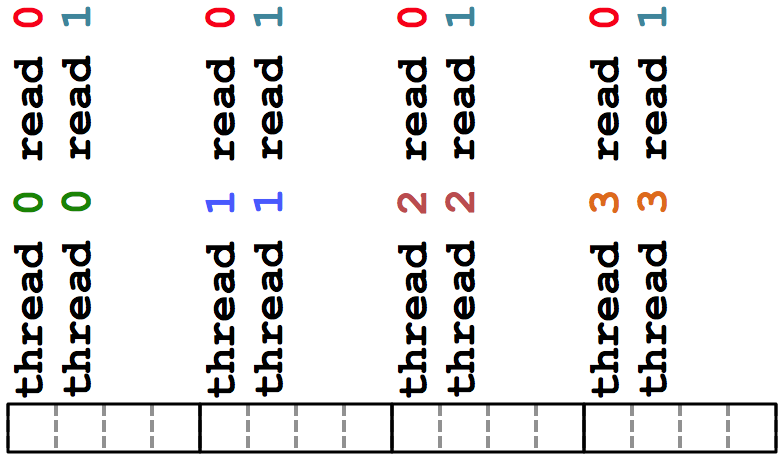
\includegraphics[width=0.80\textwidth]{figures/MemoryAccessPatterns_Caching}
      \end{center}
    \column{.50\textwidth}
      \begin{center}
        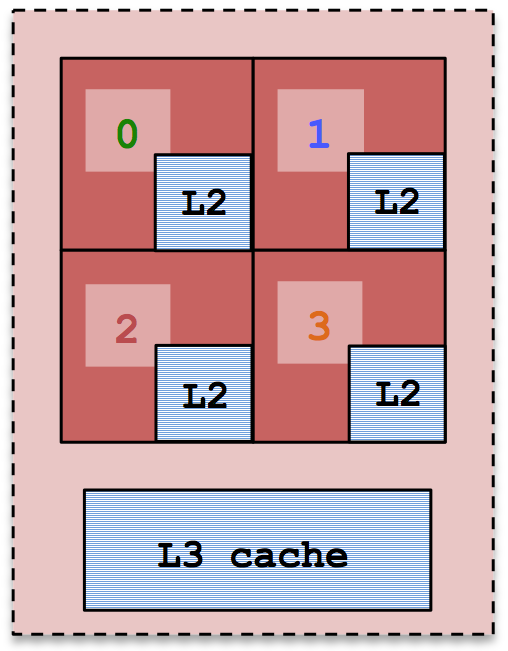
\includegraphics[width=0.38\textwidth]{figures/Schematics_CPU_withThreadIndices_justOne}
      \end{center}
  \end{columns}

  \vspace{5pt}
  \pause

  \ul{\textbf{GPUs}: many (synchronized) cores with a shared cache:}

  \vspace{-10pt}

  \begin{columns}[t,onlytextwidth]
    \column{.50\textwidth}
      \begin{center}
        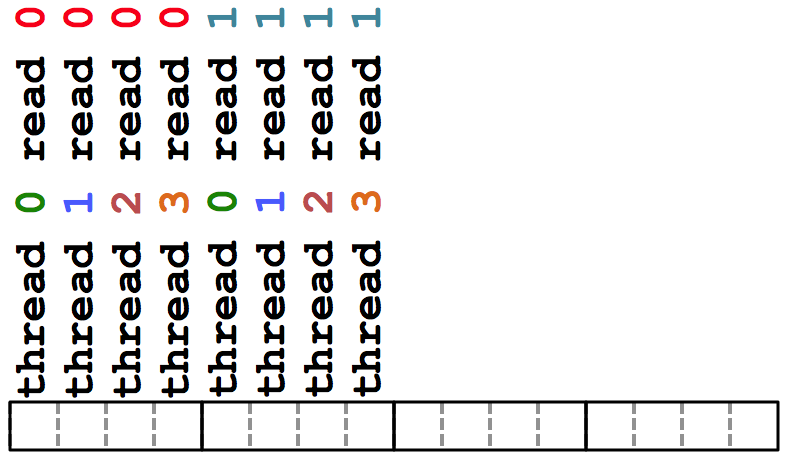
\includegraphics[width=0.80\textwidth]{figures/MemoryAccessPatterns_Coalescing}
      \end{center}
    \column{.50\textwidth}
      \begin{center}
        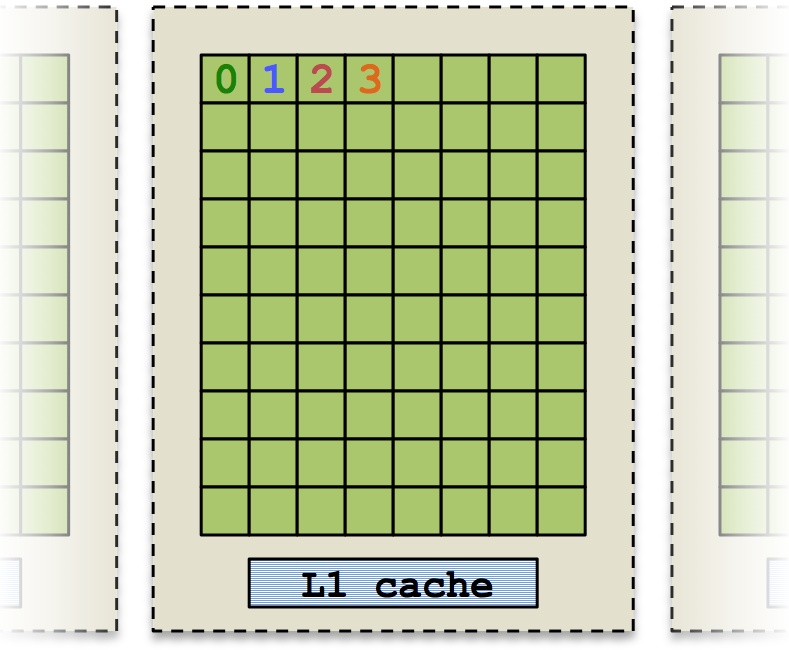
\includegraphics[width=0.60\textwidth]{figures/Schematics_GPU_withThreadIndices}
      \end{center}
  \end{columns}

\end{frame}
\fi

%==========================================================================

\begin{frame}[fragile]{Caching and coalescing (2)}

  \begin{block}{Important point}
    For performance, accesses to views in \texttt{HostSpace} must be \textbf{cached}, while access to views in \texttt{CudaSpace} must be \textbf{coalesced}.
  \end{block}

  \vspace{5pt}

  \textbf{Caching}: if thread \texttt{t}'s current access is at position \texttt{i}, \\
  \hspace{20pt} thread \texttt{t}'s next access should be at position \texttt{i+1}.

  \vspace{5pt}

  \textbf{Coalescing}: if thread \texttt{t'}s current access is at position \texttt{i}, \\
  \hspace{20pt} thread \texttt{t+1}'s current access should be at position \texttt{i+1}.

  \pause

  \begin{alertblock}{Warning}
    Uncoalesced access on GPUs and non-cached loads on CPUs \emph{greatly} reduces performance (can be 10X)
  \end{alertblock}

\end{frame}

%==========================================================================

\ifmedium
\begin{frame}[fragile]{Mapping indices to cores (0)}

  Consider the array summation example:

  \begin{code}[keywords={}]
View<double*, @boldSpace@bold> data("data", size);
...populate data...

double sum = 0;
Kokkos::parallel_reduce("Label", 
  RangePolicy< @boldSpace@bold>(0, size),
  KOKKOS_LAMBDA (const size_t index, double & valueToUpdate) {
    valueToUpdate += data(index);
  },
  sum);
  \end{code}

  \vspace{0pt}

  Question: is this cached (for \texttt{OpenMP}) and coalesced (for \texttt{Cuda})?

  \pause
  \vspace{5pt}

  Given \texttt{P} threads, \textbf{which indices} do we want thread 0 to handle?

  \vspace{-15pt}

  \begin{columns}[t,onlytextwidth]
    \column{.50\textwidth}
      \begin{center}
        Contiguous: \\
        \texttt{0, 1, 2, ..., N/P}
      \end{center}
    \column{.50\textwidth}
      \begin{center}
        Strided: \\
        \texttt{0, N/P, 2*N/P, ...}
      \end{center}
  \end{columns}

  \vspace{-10pt}
  \pause

  \begin{columns}[t,onlytextwidth]
    \column{.50\textwidth}
      \begin{center}
        \textbf{CPU}
      \end{center}
    \column{.50\textwidth}
      \begin{center}
        \textbf{GPU}
      \end{center}
  \end{columns}

  \vspace{-10pt}

  \begin{center}
    \textbf{Why?}
  \end{center}

  \vspace{-10pt}

\end{frame}
\fi

%==========================================================================

\ifmedium
\begin{frame}[fragile]{Mapping indices to cores (1)}

  \ul{\textbf{Iterating for the execution space:}}

  \begin{code}[keywords={}]
operator()(int index, double & valueToUpdate) const {
  const double d = _data(index);
  valueToUpdate += d;
}
  \end{code}

  \vspace{5pt}

  As users we don't control how indices are mapped to threads, so how do we achieve good memory access?

  \pause
  \vspace{3pt}

  \begin{block}{Important point}
    Kokkos maps indices to cores in \textbf{contiguous chunks} on CPU execution spaces, and \textbf{strided} for \texttt{Cuda}.
  \end{block}

\end{frame}
\fi

%==========================================================================

\begin{frame}[fragile]{Mapping indices to cores (2)}

  \begin{block}{Rule of Thumb}
    Kokkos index mapping and default layouts provide efficient access if \textbf{iteration indices} correspond to the \textbf{first index} of array.
  \end{block}

  \vspace{10pt}

  \textbf{Example:}

  \vspace{5pt}

  \begin{code}[keywords={}, frame=single]
  View<double***, ...> view(...);
  ...
  Kokkos::parallel_for("Label", ... ,
    KOKKOS_LAMBDA (int workIndex) {
      ...
      @darkredview(..., ... , workIndex ) = ...@darkred;
      @darkredview(... , workIndex, ... ) = ...@darkred;
      @darkgreenview(workIndex, ... , ... ) = ...@darkgreen;
    });
  ...
  \end{code}

\end{frame}

%==========================================================================

\iffull
\begin{frame}[fragile]{Example: inner product (2)}

  \begin{block}{Important point}
    Performant memory access is achieved by Kokkos mapping parallel work indices \textbf{and} multidimensional array layout \emph{appropriately for the architecture}.
  \end{block}

  \pause
  \vspace{3pt}

  \ul{\textbf{Analysis: row-major} (\texttt{LayoutRight})}

  \vspace{-10pt}

  \begin{center}
    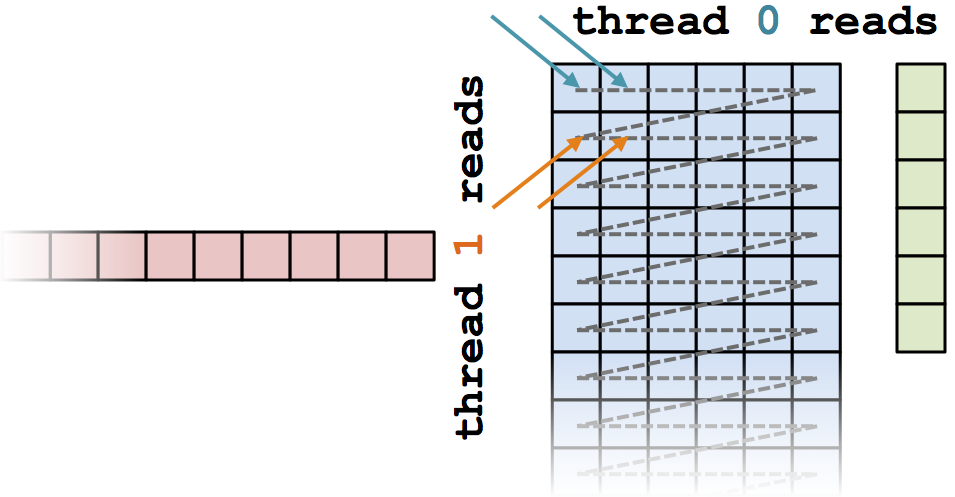
\includegraphics[width=0.65\textwidth]{figures/InnerProductExample_LayoutRight_withThreadReads}
  \end{center}

  \vspace{-28pt}
  \pause

  \begin{itemize}
    \item{\textbf{HostSpace}: cached ({\color{darkgreen}good})}
    \item{\textbf{CudaSpace}: uncoalesced ({\color{red}bad})}
  \end{itemize}

\end{frame}
\fi
\setcounter{subfigure}{0}% Reset subfigure counter


%==========================================================================

\ifmedium
\begin{frame}[fragile]{Example: inner product (3)}

  \begin{block}{Important point}
    Performant memory access is achieved by Kokkos mapping parallel work indices \textbf{and} multidimensional array layout \emph{optimally for the architecture}.
  \end{block}

  \vspace{3pt}

  \ul{\textbf{Analysis: column-major} (\texttt{LayoutLeft})}

  \vspace{-10pt}

  \begin{center}
    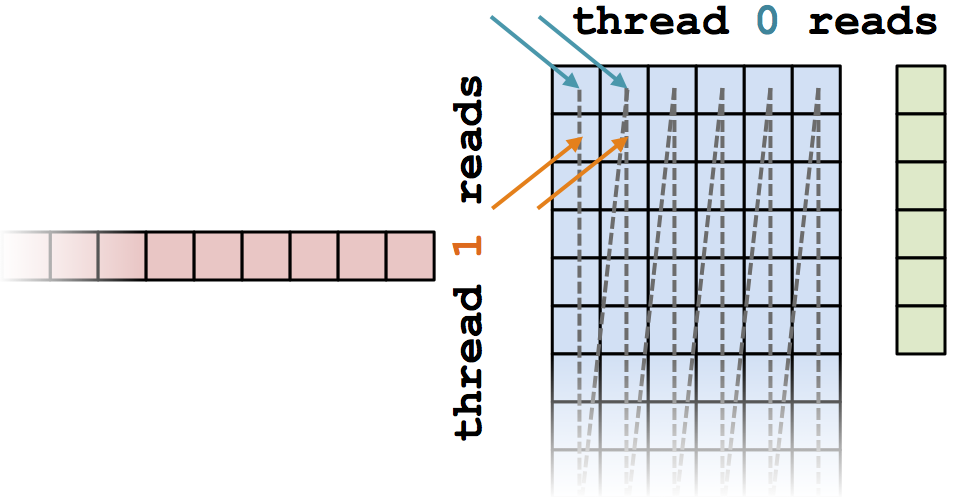
\includegraphics[width=0.65\textwidth]{figures/InnerProductExample_LayoutLeft_withThreadReads}
  \end{center}

  \vspace{-28pt}
  \pause

  \begin{itemize}
    \item{\textbf{HostSpace}: uncached ({\color{red}bad})}
    \item{\textbf{CudaSpace}: coalesced ({\color{darkgreen}good})}
  \end{itemize}

\end{frame}
\fi
\setcounter{subfigure}{0}% Reset subfigure counter

%==========================================================================

\begin{frame}[fragile]{Example: inner product (4)}

  \ul{\textbf{Analysis: Kokkos architecture-dependent}}

  \vspace{-3pt}

  \begin{code}[keywords={}]
View<double**, @boldExecutionSpace@bold> @blueA@blue(N, M);
parallel_for(RangePolicy< @boldExecutionSpace@bold>(0, N),
  ... thisRowsSum += @blueA@blue(j, i) * @darkgreenx@darkgreen(i);
  \end{code}

  \vspace{-20pt}

  \begin{figure}
    \centering
    \subfloat[\texttt{OpenMP}]{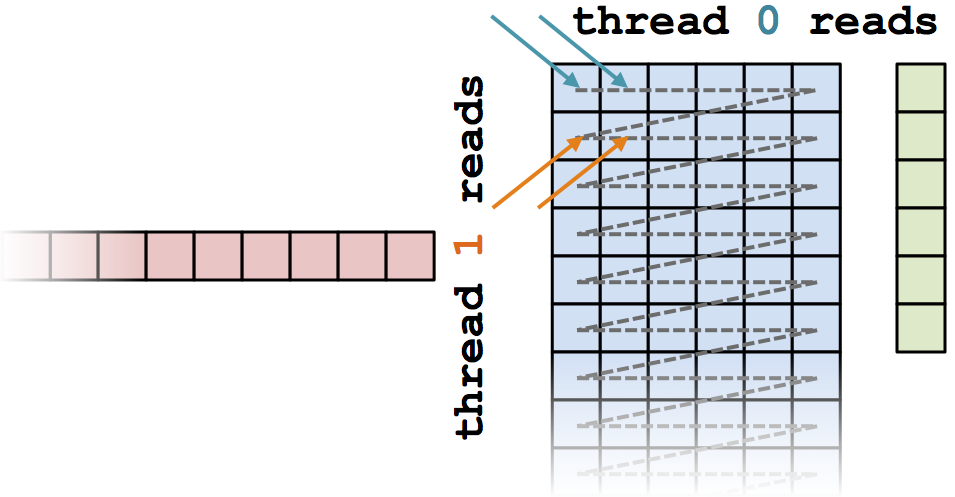
\includegraphics[trim=450pt 0pt 0pt 0pt, clip,width=0.30\textwidth]{figures/InnerProductExample_LayoutRight_withThreadReads}} \qquad
    \subfloat[\texttt{Cuda}]{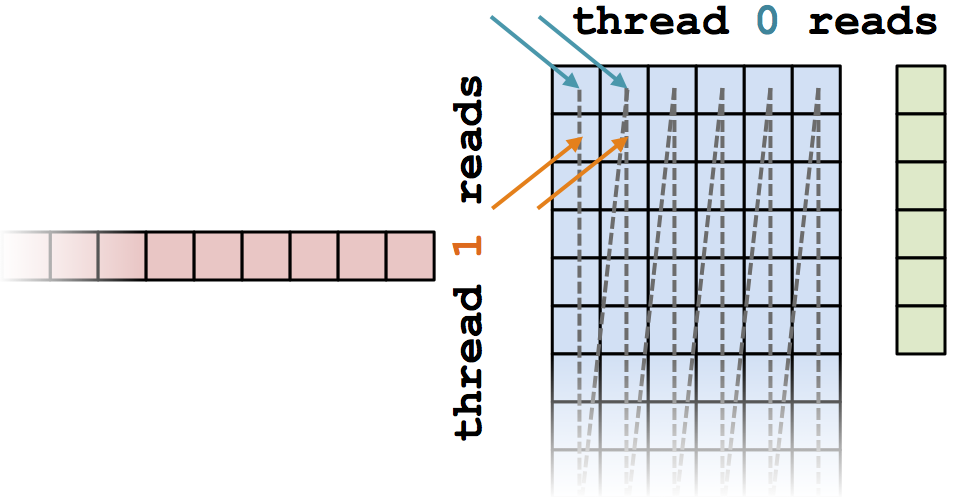
\includegraphics[trim=450pt 0pt 0pt 0pt, clip,width=0.30\textwidth]{figures/InnerProductExample_LayoutLeft_withThreadReads}}
  \end{figure}

  \vspace{-10pt}

  \begin{itemize}
    \item{\textbf{HostSpace}: cached ({\color{darkgreen}good})}
    \item{\textbf{CudaSpace}: coalesced ({\color{darkgreen}good})}
  \end{itemize}

\end{frame}
\setcounter{subfigure}{0}% Reset subfigure counter

%==========================================================================

\begin{frame}[fragile]{Example: inner product (5)}

  \vspace{-10pt}

    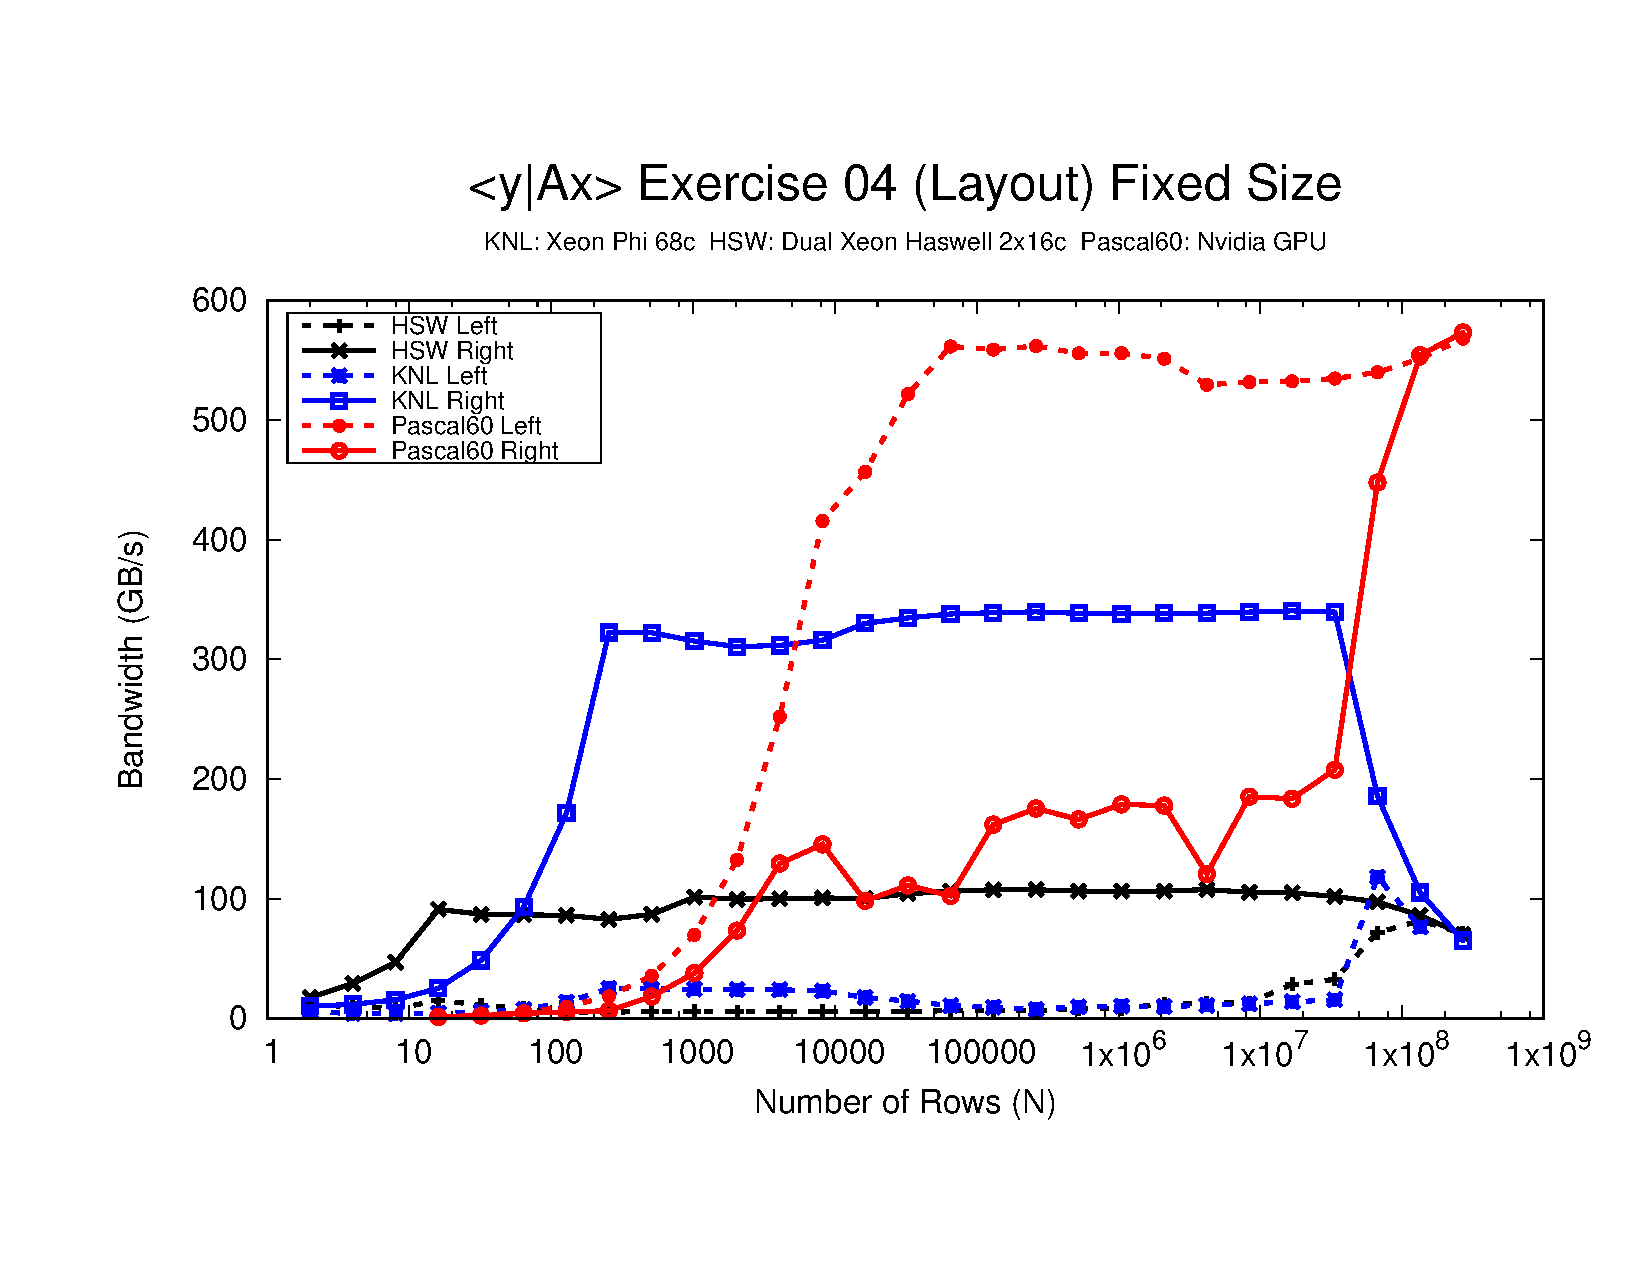
\includegraphics[viewport=1.25in 3.0in 10in 6in, width=0.95\textwidth]{figures/Exercise04-Performance.pdf}

  \vspace{-15pt}

  \begin{textblock*}{0.5\textwidth}(0.65\textwidth,0.28\textheight)
    \textbf{coalesced}
  \end{textblock*}

  \begin{textblock*}{0.5\textwidth}(0.60\textwidth,0.44\textheight)
    \textbf{cached}
  \end{textblock*}

  \begin{textblock*}{0.5\textwidth}(0.60\textwidth,0.61\textheight)
    \textbf{uncoalesced}
  \end{textblock*}

  \begin{textblock*}{0.5\textwidth}(0.70\textwidth,0.72\textheight)
    \textbf{cached}
  \end{textblock*}

  \begin{textblock*}{0.5\textwidth}(0.70\textwidth,0.77\textheight)
    \textbf{uncached}
  \end{textblock*}

\end{frame}

%==========================================================================

\begin{frame}{Memory Access Pattern Summary}

  \begin{itemize}
    \item{Every \texttt{View} has a \texttt{Layout} set at compile-time through a \textbf{template parameter}.}
    \item{\texttt{LayoutRight} and \texttt{LayoutLeft} are \textbf{most common}.}
    \item{\texttt{Views} in \texttt{HostSpace} default to \texttt{LayoutRight} and \texttt{Views} in \texttt{CudaSpace} default to \texttt{LayoutLeft}.}
    \item{Layouts are \textbf{extensible} and \textbf{flexible}.}
    %\item{Correct memory access pattern is \textbf{essential} for performance.}
    \item{For performance, memory access patterns must result in \textbf{caching} on a CPU and \textbf{coalescing} on a GPU.}
    \item{Kokkos maps parallel work indices \textit{and} multidimensional array layout for \textbf{performance portable memory access patterns}.}
    \item{There is \textbf{nothing in} \texttt{OpenMP}, \texttt{OpenACC}, or \texttt{OpenCL} to manage layouts.}\\
    $\Rightarrow$ You'll need multiple versions of code or pay the performance penalty.
  \end{itemize}

\end{frame}



\begin{frame}[fragile]{}

  {\Huge Advanced Reductions}

  \vspace{20pt}

  \textbf{Learning objectives:}
  \begin{itemize}
    \item{How to use Reducers to perform different reductions.}
    \item{How to do multiple reductions in one kernel.}
    \item{Using \texttt{Kokkos::View}'s as result for asynchronicity.}
    \item{Custom reductions}
  \end{itemize}

  \vspace{-20pt}

\end{frame}

\begin{frame}[fragile]{Reducers}

\textbf{So far only "sum" reduction. What about other things?}

\textbf{Using a Reducer:}
\begin{code}[linebackgroundcolor={
          \btLstHL<2>{5}{red!20}
        }, keywords={parallel_reduce,double,Max}]
double max_value = 0;
parallel_reduce("Label", numberOfIntervals,
  KOKKOS_LAMBDA(const int64_t i, double & valueToUpdate) {
    double my_value = function(...);
    if(my_value > valueToUpdate) valueToUpdate = my_value;
}, Kokkos::Max<double>(max_value));
\end{code}

\begin{itemize}
\item<2-> Note how the operation in the body matches the reducer op!
\item<3-> The scalar type is used as a template argument.
\item<4-> Many reducers available: \texttt{Sum, Prod, Min, Max, MinLoc,} see:  {\tiny \url{https://kokkos.github.io/kokkos-core-wiki/API/core/builtin_reducers.html}}
\item<5-> Some reducers (like \texttt{MinLoc}) use special scalar types!
\item<6-> Custom value types supported via specialization of \texttt{reduction\_identity}.
\end{itemize}
\end{frame}

\begin{frame}[fragile]{Simultaneous Reductions}

\textbf{Sometimes multiple reductions are needed}

	\begin{itemize}
		\item Provide multiple reducers/result arguments
		\item Functor/Lambda operator takes matching thread-local variables
		\item Mixing scalar types is fine.
	\end{itemize}

\begin{code}[keywords={parallel_reduce,double,float,Max}]
float max_value = 0;
double sum = 0;
parallel_reduce("Label", numberOfIntervals,
    KOKKOS_LAMBDA(const int64_t i,float& tl_max,double& tl_sum){
  float a_i = a[i];
  if(a_i > tl_max) tl_max = a_i;
  tl_sum += a_i;
}, Kokkos::Max<float>(max_value),sum);
\end{code}

\end{frame}

\begin{frame}[fragile]{Views as Result arguments}

\textbf{Reducing into a Scalar is blocking!}

	\begin{itemize}
		\item Providing a reference to scalar means no lifetime expectation.
			\begin{itemize}
				\item Call to \texttt{parallel\_reduce} returns after writing the result.
			\end{itemize}
		\item \texttt{Kokkos::View} can be used as a result, allowing for potentially non-blocking execution.
		\item Can provide \texttt{View} to host memory, or to memory accessible by the \texttt{ExecutionSpace} for the reduction.
		\item Works with Reducers too!
	\end{itemize}

	\begin{code}[keywords={parallel_reduce,double,View,RangePolicy,CudaSpace,HostSpace}]
View<double,HostSpace> h_sum("sum_h");
View<double,CudaSpace> d_sum("sum_d");
using policy_t = RangePolicy<Cuda>;

parallel_reduce("Label", policy_t(0,N), SomeFunctor, 
  h_sum);

parallel_reduce("Label", policy_t(0,N), SomeFunctor, 
  Kokkos::Sum<double,CudaSpace>(d_sum));
\end{code}
\end{frame}

\begin{frame}[fragile]{Custom Reductions}
\textbf{Pseudocode for Kokkos implementation}
\begin{code}[keywords={parallel_reduce,custom}]
per_thread:
  value& tmp=init(local_tmp);
  for (i in local range)
    functor(i, tmp)
call join for merging values between threads
  in the same thread group
let one (the last) thread group merge all results
  from all thread groups
call final(result) on one thread 
\end{code}

Three ingredients
\begin{itemize}
\item init (optional), default: default constructor
\item join (required)
\item final (optional), default: no-op
\end{itemize}

\end{frame}

\begin{frame}[fragile]{Custom Reductions}
Rules for choosing reduction behavior
\begin{enumerate}
\item If a reducer is specified (return type is a functor with \texttt{reducer} alias to itself), use that.
\item If functor implements \texttt{join}, use functor as reducer.
\item Otherwise, assume \texttt{join} behaves like \texttt{operator+}.
\end{enumerate}

Note that the functor's \texttt{init}, \texttt{join}, \texttt{final} members must be tagged if the call operator is tagged. The reducers member functions must never be tagged.
\end{frame}

\begin{frame}[fragile]{Reducer Concept}
\scriptsize
\begin{code}[basicstyle=\tiny]
class Reducer {
  public:
    using reducer    = Reducer;
    using value_type = ... ;
    using result_view_type = Kokkos::View<value_type, ... >;

    KOKKOS_FUNCTION
    void join(value_type& dest, const value_type& src) const;

    //optional
    KOKKOS_INLINE_FUNCTION
    void init(value_type& val) const;
   
    //optional
    KOKKOS_INLINE_FUNCTION
    void final(value_type& val) const;

    KOKKOS_INLINE_FUNCTION
    value_type& reference() const;

    KOKKOS_INLINE_FUNCTION
    result_view_type view() const;

    KOKKOS_INLINE_FUNCTION
    Reducer(value_type& value_);

    KOKKOS_INLINE_FUNCTION
    Reducer(const result_view_type& value_);
};
\end{code}
\end{frame}


\begin{frame}[fragile]{Module 2: Summary}
	\textbf{Kokkos View}
	\begin{itemize}
		\item Multi Dimensional Array.
		\item Compile and Runtime Dimensions.
		\item Reference counted like a \texttt{std::shared\_ptr} to an array.
	\end{itemize}
\begin{code}[keywords={View,int}]
	Kokkos::View<int*[5]> a("A", N);
	a(3,2) = 7;
\end{code}

	\textbf{Execution Spaces}
	\begin{itemize}
		\item{Parallel operations execute in a specified \textbf{Execution Space}}
		\item{Can be controlled via template argument to \textbf{Execution Policy}}
		\item{If no Execution Space is provided use \texttt{DefaultExecutionSpace}}
	\end{itemize}
\begin{code}[keywords={parallel_for,Cuda,RangePolicy}]
// Equivalent:
parallel_for("L", N, functor);
parallel_for("L",
  RangePolicy<DefaultExecutionSpace>(0, N), functor);
\end{code}
\end{frame}

\begin{frame}[fragile]{Module 2: Summary}
	\textbf{Memory Spaces}
	\begin{itemize}
		\item Kokkos Views store data in \textbf{Memory Spaces}.
		\item Provided as template parameter.
		\item If no Memory Space is given, use  \texttt{Kokkos::DefaultExecutionSpace::memory\_space}.
		\item \texttt{deep\_copy} is used to transfer data: no hidden memory copies by Kokkos.
	\end{itemize}
\begin{code}[keywords={View,int,CudaSpace,create_mirror_view}]
	View<int*, CudaSpace> a("A", M);
	// View in host memory to load from file
	auto h_a = create_mirror_view(a);
        load_from_file(h_a);
	// Copy
	deep_copy(a,h_a);
\end{code}

\end{frame}

\begin{frame}[fragile]{Module 2: Summary}
	\textbf{Layouts}
	\begin{itemize}
		\item Kokkos Views use an index mapping to memory determined by a \textbf{Layout}.
		\item Provided as template parameter.
		\item If no \textbf{Layout} is given, derived from the execution space associated with the memory space.
		\item Defaults are good if you parallelize over left most index!
	\end{itemize}

\begin{code}[keywords={View,int,CudaSpace}]
	View<int**, LayoutLeft> a("A", N, M);
	View<int**, LayoutRight> b("B", N, M);

	parallel_for("Fill", N, KOKKOS_LAMBDA(int i) {
          for(int j = 0; j < M; j++) {
            a(i,j) = i * 1000 + j; // coalesced
	    b(i,j) = i * 1000 + j; // cached
          }
	});
\end{code}

\end{frame}

\begin{frame}[fragile]{Module 2: Summary}
	\textbf{Advanced Reductions}
	\begin{itemize}
        \item \texttt{parallel\_reduce} defaults to summation
        \item Kokkos reducers can be used to reduce over arbitrary operations
        \item Reductions over multiple values are supported
        \item Only reductions into scalar arguments are guaranteed to be synchronous
        \item Support for custom reductions
	\end{itemize}

\begin{code}[keywords={View,int,CudaSpace}]
    parallel_reduce("Join", n,
      KOKKOS_LAMBDA(int i, double& a, int& b) {
        int idx = foo();
        if(idx > b) b = idx;
        a += bar();
      }, result, Kokkos::Max<int>{my_max});
\end{code}

\end{frame}

\begin{frame}{Module 3: Outlook (07/31)}

	\vspace{10pt}
	\textbf{Advanced Data Structures}
	\begin{itemize}
        \item Subsetting and slicing of \texttt{View}s
        \item Higher-level and special purpose \texttt{View} data structures
        \item Atomic access to a \texttt{View}'s data
	\end{itemize}

	\vspace{10pt}
	\textbf{More Parallel Policies:}
	\begin{itemize}
		\item Multidimensional loops with \texttt{MDRangePolicy}
	\end{itemize}

	\vspace{10pt}
    \textbf{Slack channel:} {\scriptsize \url{https://kokkosteam.slack.com/}}
	
	\vspace{10pt}
	\textbf{Recordings/Slides:} {\scriptsize \url{https://kokkos.org/kokkos-core-wiki/videolectures.html}}

\end{frame}

\end{document}

